\documentclass[a4paper]{report}
\usepackage{geometry}
\usepackage{graphics}
\usepackage{ifpdf}
% \usepackage{makeidx}
\usepackage{fancyhdr}
\usepackage{fancyvrb}
\usepackage{amsmath, amsthm, amssymb}
\usepackage{graphicx}
\usepackage{tikz}

\ifpdf
\pdfinfo{
  /Title    (Clus: User's Manual)
  /Author   (Jan Struyf, Bernard Zenko, Hendrik Blockeel, Celine Vens, Matej Petkovic, Tomaz Stepisnik Perdih, Vanja Mileski, Martin Breskvar, Jurica Levatic, Dragi Kocev, Saso Dzeroski)
}
\usepackage[pdftex,colorlinks=true,pdfstartview=FitV,linkcolor=black,citecolor=black,urlcolor=black]{hyperref}
\else
\usepackage{url}
\newcommand{\phantomsection}[1]{}
\fi

% geometry makes sure page size is correct in .pdf files
\geometry{a4paper,
          centering,
          textwidth = 16.5cm,
          textheight = 24.5cm
}

\renewcommand{\topfraction}{1.0}
\setcounter{topnumber}{4}
\setcounter{totalnumber}{4}
\renewcommand{\textfraction}{0.07}

\newcommand{\clus}{\textsc{Clus}}
\newcommand{\clusphy}{\textsc{Clus}-$\varphi$}
%\newcommand{\comment}[1]{{\color{red}\textbf{COMMENT:} #1}}
\newcommand{\comment}[1]{} % off

% commands for option lists
\newcommand{\optionNameStyle}[1]{{\tt #1}}
\newcommand{\optionPossibleValues}{\emph{possible values}}
\newcommand{\optionDefaultValue}{\emph{default}}
\newcommand{\optionDefaultValueStyle}[1]{{\tt #1}}
\newcommand{\optionDescrption}[1]{{\it description #1}}


\def\trim#1{\ignorespaces#1\unskip}
\newcommand{\optionPossibleValuesList}[1]{%
	\listItems{#1}%
}
\newcommand{\formatOneElement}[1]{\texttt{\trim{#1}}}
\def\listItems#1{%
	\gdef\firstelement{1}
	\{%
	\foreach \e [count=\ni] in {#1}{%
		\ifnum\firstelement=0, \fi%
		\formatOneElement{\e}%
		\gdef\firstelement{0}%
	}%
	\}%
}


\newcommand{\doNotShowThis}[1]{}



\begin{document}

\title{\clus: User's Manual}

\author{Jan Struyf, Bernard \v{Z}enko, Hendrik Blockeel, Celine Vens,\\ Matej Petkovi\'{c}, Toma\v{z} Stepi\v{s}nik Perdih, Vanja Mileski,\\ Martin Breskvar, Jurica Levati\'{c}, Dragi Kocev, Sa\v{s}o D\v{z}eroski}


\maketitle


\tableofcontents

%
%%%%%%%%%%%%%%%%%%%%%
\chapter{Introduction}

This text is a user's manual for the open source machine learning system \clus{}. \clus{} is a decision tree and rule learning system that works in the \emph{predictive clustering} framework \cite{Blockeel1998icml}.
% Should we avoid one (or two) sentence paragraphs?
While most decision tree learners induce classification or regression trees, \clus{} generalizes this approach by learning trees that are interpreted as cluster hierarchies. We call such trees predictive clustering trees or PCTs. Depending on the learning task at hand, different goal criteria are to be optimized while creating the clusters, and different heuristics will be suitable to achieve this.

Classification and regression trees are special cases of PCTs, and by choosing the right parameter settings \clus{} can closely mimic the behavior of tree learners such as CART \cite{Breiman1984} or C4.5 \cite{Quinlan1993}.  However, its applicability goes well beyond classical classification or regression tasks: \clus{} has been successfully applied to many different tasks including multi-task learning (multi-target classification and regression), structured output learning, multi-label classification, hierarchical classification, hierarchical regression, and time series prediction. Next to these supervised learning tasks, PCTs are also applicable to semi-supervised learning, subgroup discovery, and clustering.
%
In a similar way, predictive clustering rules (PCRs) generalize classification rule sets \cite{Clark91:proc} and also apply to the aforementioned learning tasks.

A full description of how \clus{} works is beyond the scope of this text. In this User's Manual, we focus on how to use \clus{}: how to prepare its inputs, how to interpret the outputs, and how to change its behavior with the available parameters. This manual is a work in progress and all comments are welcome.
%
For background information on the rationale behind the \clus{} system and its algorithms we refer the reader to the following papers:

\begin{itemize} 

\item H.~Blockeel, L.~De Raedt, and J.~Ramon.
\newblock Top-down induction of clustering trees.
\newblock In \emph{Proceedings of the 15th International Conference on Machine
  Learning}, pages 55--63, 1998.

\item H.~Blockeel and J.~Struyf.
\newblock Efficient algorithms for decision tree cross-validation.
\newblock \emph{Journal of Machine Learning Research}, 3: 621--650,
  December 2002.

\item H. Blockeel, S. D\v zeroski, and J. Grbovi\'c, Simultaneous prediction of multiple chemical parameters of river water quality with TILDE, Proceedings of the Third European Conference on Principles of Data Mining and Knowledge Discovery (J.M. \.{Z}ytkow and J. Rauch, eds.), vol 1704, LNAI, pp. 32-40, 1999.

\item T.~Aho, B.~{\v{Z}}enko, and S.~D{\v{z}}eroski.
\newblock Rule ensembles for multi-target regression.
\newblock In \emph{Proceedings of 9th IEEE International Conference on Data
  Mining (ICDM 2009)}, pages 21--30, 2009.

\item E.~Fromont, H.~Blockeel, and J.~Struyf.
\newblock Integrating decision tree learning into inductive databases.
\newblock \emph{Lecture Notes in Computer Science}, 4747: 81--96,
  2007.

\item D.~Kocev, C.~Vens, J.~Struyf, and S.~D{\v{z}}eroski.
\newblock Ensembles of multi-objective decision trees.
\newblock \emph{Lecture Notes in Computer Science}, 4701: 624--631,
  2007.

\item I.~Slavkov, V.~Gjorgjioski, J.~Struyf, and S.~D{\v z}eroski.
\newblock Finding explained groups of time-course gene expression profiles with
  predictive clustering trees.
\newblock \emph{Molecular Biosystems}, 2009.
\newblock To appear.

\item J.~Struyf and S.~D\v{z}eroski.
\newblock Clustering trees with instance level constraints.
\newblock \emph{Lecture Notes in Computer Science}, 4701: 359--370,
  2007.

\item J.~Struyf and S.~D{\v{z}}eroski.
\newblock Constraint based induction of multi-objective regression trees.
\newblock \emph{Lecture Notes in Computer Science}, 3933: 110--121,
  2005.

\item C.~Vens, J.~Struyf, L.~Schietgat, S.~D{\v z}eroski, and H.~Blockeel.
\newblock Decision trees for hierarchical multi-label classification.
\newblock \emph{Machine Learning}, 73 (2): 185--214, 2008.

\item B.~{\v{Z}}enko and S.~D{\v{z}}eroski.
\newblock Learning classification rules for multiple target attributes.
\newblock In \emph{Advances in Knowledge Discovery and Data Mining}, pages
  454--465, 2008.

\end{itemize}

A longer list of publications describing different aspects and applications of \clus{} is available on the \clus{} web site
(\url{www.cs.kuleuven.be/~dtai/clus/publications.html}).

%
%%%%%%%%%%%%%%%%%%%%%%%%
\chapter{Getting Started}

\section{Installing and Running \clus}
\label{sec:run}

\begin{sloppypar}
\clus{} is written in the Java programming language, which is available from {\tt http://java.sun.com}. You will need Java version 1.5.x or newer. To run \clus{}, it suffices to install the Java Runtime Environment (JRE). If you want to make changes to \clus{} and compile its source code, then you will need to install the Java Development Kit (JDK) instead of the JRE.
\end{sloppypar}

The \clus\ software is released under the GNU General Public License version 3 or later and is available for download at \url{http://www.cs.kuleuven.be/~dtai/clus/}. After downloading \clus{}, unpack it into a directory of your choice. \clus{} is a command line application and should be started from the command prompt (Windows) or a terminal window (Unix). To start \clus{}, enter the command:
\begin{flushleft}
\verb^java -jar $CLUS_DIR/Clus.jar^ {\em filename}\verb^.s^
\end{flushleft}

\noindent{}with \verb^$CLUS_DIR/Clus.jar^ the location of \verb^Clus.jar^ in your \clus{} distribution and {\tt {\em filename}.s} the name of your settings file. In order to verify that your \clus\ installation is working properly, you might try something like:

\begin{list}{\labelitemi}{\leftmargin=1.5cm}
\item[Windows:]\mbox{}
\begin{verbatim}
cd C:\Clus\data\weather
java -jar ..\..\Clus.jar weather.s
\end{verbatim}

\item[Unix:]\mbox{}
\begin{verbatim}
cd $HOME/Clus/data/weather
java -jar ../../Clus.jar weather.s
\end{verbatim}
\end{list}

\noindent{}This runs \clus{} on a simple example \emph{Weather.} You can also try other example data sets in the \texttt{data} directory of the \clus{} distribution.

Note that the above instructions are for running the pre-compiled version of \clus{} (\texttt{Clus.jar}), which is included with the \clus{} download. If you have modified and recompiled \clus{}, or if you are using the SVN developers version, then you should run \clus{} in a different way, as is explained in Chapter~\ref{ch:devel}.

%
%%%%%%%%%%%%%%%%%%%%%%%%%%%%%%%%%%%%%%%%%
\section{Input and Output Files for \clus}

\begin{figure}%[tb]
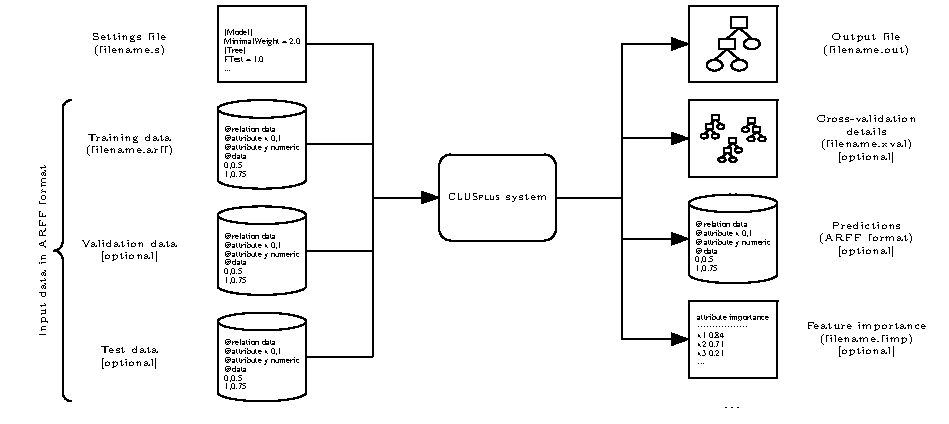
\includegraphics{fig/clusinout}
\caption{\label{fig:iofiles}Input and output files of \clus.}
% .xval and predictions are not always produced - should we mention this in the figure?
\end{figure}

\begin{figure}%[tb]
\hrule\vspace{1em}
\begin{verbatim}
[Attributes]
Descriptive = 1-2
Target = 3-4
Clustering = 3-4

[Tree]
Heuristic = VarianceReduction
\end{verbatim}
\hrule
\caption{The settings file (\texttt{weather.s}) for the \emph{Weather} example.}
\label{weathers:fig}
\end{figure}
\begin{figure}%[tb]
\hrule\vspace{1em}
\begin{verbatim}
@RELATION "weather"

@ATTRIBUTE outlook     {sunny,rainy,overcast}
@ATTRIBUTE windy       {yes,no}
@ATTRIBUTE temperature numeric
@ATTRIBUTE humidity    numeric

@DATA
sunny,    no,  34, 50
sunny,    no,  30, 55
overcast, no,  20, 70 
overcast, yes, 11, 75
rainy,    no,  20, 88
rainy,    no,  18, 95 
rainy,    yes, 10, 95 
rainy,    yes, 8,  90
\end{verbatim}
\hrule
\caption{The training data (\texttt{weather.arff}) for the \emph{Weather} example (in Weka's ARFF format).}
\label{weatherarff:fig}
\end{figure}

\begin{figure}[tb]
\hrule\vspace{1em}
\begin{verbatim}
Clus run "weather"
******************
Date: 1/10/10 12:23 PM
File: weather.out
Attributes: 4 (input: 2, output: 2)

[Data]
File = weather.arff

[Attributes]
Target = 3-4
Clustering = 3-4
Descriptive = 1-2

[Tree]
Heuristic = VarianceReduction
PruningMethod = M5

Statistics
----------
Induction Time: 0.017 sec
Pruning Time: 0.001 sec
Model information
     Original: Nodes = 7 (Leaves: 4)
     Pruned: Nodes = 3 (Leaves: 2)

Training error
--------------
Number of examples: 8
Mean absolute error (MAE)
   Default        : [7.125,14.75]: 10.9375
   Original       : [2.125,2.75]: 2.4375
   Pruned         : [4.125,7.125]: 5.625
Mean squared error (MSE)
   Default        : [76.8594,275.4375]: 176.1484
   Original       : [6.5625,7.75]: 7.1562
   Pruned         : [19.4375,71.25]: 45.3438

Original Model
**************
outlook = sunny
+--yes: [32,52.5]: 2
+--no:  outlook = rainy
        +--yes: windy = yes
        |       +--yes: [9,92.5]: 2
        |       +--no:  [19,91.5]: 2
        +--no:  [15.5,72.5]: 2

Pruned Model
************
outlook = sunny
+--yes: [32,52.5]: 2
+--no:  [14.5,85.5]: 6
\end{verbatim}
\hrule
\caption{The \emph{Weather} example's output (\texttt{weather.out}). (Some parts have been omitted for brevity.)}
\label{weatherout:fig}
\end{figure}

\clus{} uses (at least) two input files and these are named {\tt {\em filename}.s} and {\tt {\em filename}.arff}, with {\tt {\em filename}} a name chosen by the user.  The file {\tt {\em filename}.s} contains the parameter settings for \clus{}. The file {\tt {\em filename}.arff} contains the training data to be read. The format of the data file is Weka's ARFF format\footnote{\url{http://weka.wikispaces.com/ARFF}}. The results of a \clus{} run are put in an output file {\tt {\em filename}.out}. Figure~\ref{fig:iofiles} gives an overview of the input and output files supported by \clus{}. The format of the data files is described in detail in Chapter~\ref{ch:data}, the format of the settings file is discussed in Chapter~\ref{ch:sett}, and the output files are covered in Chapter~\ref{ch:output}. Optionally, \clus\ can also generate a detailed output of the cross-validation (\texttt{weather.xval}) and model predictions in ARFF format.

%
%%%%%%%%%%%%%%%%%%%%%%%%%%%%%%%
\section{A Step-by-step Example}

The \clus{} distribution includes a number of example datasets.  In this section we briefly take a look at the {\em Weather} dataset, and how it can be processed by \clus{}.  We use Unix notation for paths to filenames; in Windows notation the slashes become backslashes (see also previous section).
\begin{enumerate}
  \item Move to the directory {\tt Clus/data/weather}, which contains the {\em Weather} dataset:
\begin{verbatim}
cd Clus/data/weather
\end{verbatim}

  \item First inspect the file {\tt weather.arff}.  Its contents is also shown in Figure~\ref{weatherarff:fig}.
This file contains the input data that \clus{} will learn from.  It is in the ARFF format: first, the name of the table is given; then, the attributes and their domains are listed; finally, the table itself is listed.

  \item Next, inspect the file {\tt weather.s}.  This file is also shown in Figure~\ref{weathers:fig}.  
It is the {\em settings} file, the file where \clus{} will find information about the task it should perform, values for its parameters, and other information that guides it behavior.

%In the \emph{Weather} example of Section~\ref{sec:run}, \clus{} will read its settings from the input file \texttt{weather.s} (shown in Figure~\ref{weathers:fig}) and its input data from the file \texttt{weather.arff} (Figure~\ref{weatherarff:fig}). It will then construct (with these settings) a PCT, which it will write to the output file \texttt{weather.out} (Figure~\ref{weatherout:fig}).

The \emph{Weather} example is a small multi-target or multi-task learning problem \cite{Caruana97:jrnl}, in which the goal is to predict the target attributes \emph{temperature} and \emph{humidity} from the input attributes \emph{outlook} and \emph{windy.}  This kind of information is what goes in the settings file.
% Our example includes values for four parameters. 
The parameters under the heading \texttt{[Attributes]} specify the role of the different attributes. In our learning problem, the first two attributes (attributes 1-2: \emph{outlook} and \emph{windy}) are \emph{descriptive} attributes: they are to be used in the cluster descriptions, that is, in the tests that appear in the predictive clustering tree's nodes (or, in rule learning, the conditions that appear in predictive clustering rules). The last two attributes (attributes 3-4) are so-called {\em target} attributes: these are to be predicted from the descriptive attributes. The setting \texttt{Clustering = 3-4} indicates that the clustering heuristic, which is used to construct the tree, should be computed based on the target attributes only.  (That is, \clus{} should try to produce clusters that are coherent with respect to the target attributes, not necessarily with respect to all attributes.)
Finally, in the {\tt Tree} section of the settings file, which contains parameters specific to tree learning, \texttt{Heuristic = VarianceReduction} specifies that, among different clustering heuristics that are available, the heuristic that should be used for this run is variance reduction. 

These are only a few possible settings.  Chapter~\ref{ch:sett} provides a detailed description of each setting supported by \clus{}.  

  \item Now that we have some idea of what the settings file and data file look like, let's run \clus{} on these data and see what the result is.  From the Unix command line, type, in the directory where the weather files are:
\begin{verbatim}
java -jar ../../Clus.jar weather.s
\end{verbatim}

  \item \clus{} now reads the data and settings files, performs it computations, and writes the resulting predictive clustering tree, together with a number of statistics such as the training set error and the test set error (if a test set has been provided), to an output file, {\tt weather.out}.  Open that file and inspect its contents; it should look like the file shown in Figure~\ref{weatherout:fig}.  The file contains information about the \clus{} run, including some statistics, and of course also the final result: the predictive clustering tree that we wanted to learn.  By default, \clus{} shows both an ``original model'' (the tree before pruning it) and a ``pruned model'', which is a simplified version of the original one.

In this example, the resulting tree is a multi-target tree: each leaf predicts a vector of which the first component is the predicted \emph{temperature} (attribute 3) and the second component the predicted \emph{humidity} (attribute 4).  A feature that distinguishes \clus{} from other decision tree learners is exactly the fact that \clus{} can produce this kind of trees.  Constructing a multi-target tree has several advantages over constructing a separate regression tree for each target variable. The most obvious one is the number of models: the user only has to interpret one tree instead of one tree for each target. A second advantage is that the tree makes features that are relevant to all target variables explicit. For example, the first leaf of the tree in Figure~\ref{weatherout:fig} shows that \texttt{outlook = sunny} implies both a high temperature and a low humidity. Finally, due to so-called inductive transfer, multi-target PCTs may also be more accurate than regression trees. More information about multi-target trees can be found in the following publications: \cite{Blockeel1998icml, Blockeel99:proc, Struyf06-KDID:proc, Piccart08-DS:proc}.

\end{enumerate}
% \chapter{Learning Algorithms}
% 
% \section{Tree Learning}
% 
% \subsection{Top-down Induction}
% 
% \subsection{Beam Search}
% 
% \subsection{Constrained Induction}
% 
% \subsection{s}
% 
% \section{Rule Learning}
% 
% \subsection{Sequential Covering Algorithm}
% 
% \subsection{Rule Ensembles}
% 
% \chapter{Case Studies}
%  
% \section{Multi-target Regression and Classification}
% 
% \section{Hierarchical Multi-label Classification}
% 
% \section{Time Series Clustering}
% 
% \section{Clustering with Instance Level Constraints}

%
%%%%%%%%%%%%%%%%%%%%%
\chapter{Input Format}
\label{ch:data}

Like many machine learning systems, \clus\ learns from tabular data. These data are assumed to be in the ARFF format that is also used by the Weka data mining tool.  Full details on ARFF can be found elsewhere\footnote{\url{http://weka.wikispaces.com/ARFF}}. We only give a minimal description here.

In the data table, each row represents an instance, and each column represents an attribute of the instances.  Each attribute has a name and a domain (the domain is the set of values it can take). In the ARFF format, the names and domains of the attributes are declared up front, before the data are given. The syntax is not case sensitive.
%
An ARFF file has the following format:

\begin{tabbing}
{\tt \% all comment lines are optional, start with \%, and can occur }\\
{\tt \% anywhere in the file}\\
\\
{\tt @RELATION} name\\
\\
{\tt @ATTRIBUTE} name domain\\
{\tt @ATTRIBUTE} name domain\\
...\\
\\
{\tt @DATA}\\
value$_1$, value$_2$, ... , value$_n$\\
value$_1$, value$_2$, ... , value$_n$\\
\end{tabbing}

\noindent The domain of an attribute can be one of:
\begin{itemize}
	\item \texttt{numeric}
	\item \texttt{\{} nomvalue$_1$, nomvalue$_2$, ... , nomvalue$_n$ \texttt{\}}
	\item \texttt{string}
	\item \texttt{hierarchical} hvalue$_1$, hvalue$_2$, ... , hvalue$_n$
	\item \texttt{timeseries}
\end{itemize}
%
The first option, \texttt{numeric} (\texttt{real} and \texttt{integer} are also legal and are treated in the same way), indicates that the domain is the set of real numbers. The second type of domain is called a discrete domain.  Discrete domains are defined by enumerating the values they contain. These values are nominal. The third domain type is \texttt{string} and can be used for attributes containing arbitrary textual values.

The fourth type of domain is called \texttt{hierarchical} (multi-label). It implies two things: first, the attribute can take as a value a \emph{set of values} from the domain, rather than just a single value; second, the domain has a hierarchical structure.  The elements of the domain are typically denoted $v_1/v_2/.../v_i$, with $i \leq d$, where $d$ is the depth of the hierarchy.  A set of such elements is denoted by just listing them, separated by \verb^@^.  This type of domain is useful in the context of hierarchical multi-label classification and is not part of the standard ARFF syntax.  

The last type of domain is \texttt{timeseries}. A time series is a fixed length series of numeric data where individual numbers are written in brackets and separated with commas. All time series of a given attribute must be of the same length. This domain type, too, is not part of the standard ARFF syntax.

The values in a	 row occur in the same order as the attributes: the $i$'th value is assigned to the $i$'th attribute.  The values must, obviously, be elements of the specified domain.  

\clus\ also supports the sparse ARFF format, where only non-zero data values are stored for the numeric attributes. The header of a sparse ARFF file is the same, but each data instance is written in curly braces and each attribute value is written as a pair of the attribute number (starting from one) and its value separated by a space; values of different attributes are separated by commas.

Figure~\ref{weatherarff:fig} shows an example of an ARFF file. An example of a table containing hierarchical multi-label attributes is shown in Figure~\ref{arffhmc:fig}, an example ARFF file with a time series attribute is shown in Figure~\ref{arfftimeser:fig}, and an example sparse ARFF file is shown in Figure~\ref{arffsparse:fig}.

\begin{figure}[tb]
\hrule\vspace{1em}
\begin{verbatim}
@RELATION HMCNewsGroups

@ATTRIBUTE word1   {1,0}
...
@ATTRIBUTE word100 {1,0}
@ATTRIBUTE class hierarchical rec/sport/swim,rec/sport/run,rec/auto,alt/atheism,...

@DATA
1,...,1,rec/sport/swim
1,...,1,rec/sport/run
1,...,1,rec/sport/run@rec/sport/swim
1,...,0,rec/sport
1,...,0,rec/auto
0,...,0,alt/atheism
...
\end{verbatim}
\hrule\vspace{1em}
\caption{An ARFF file that includes a hierarchical multi-label attribute.}
\label{arffhmc:fig}
\end{figure}

\begin{figure}[tb]
\hrule\vspace{1em}
\begin{verbatim}
@RELATION GeneExpressionTimeSeries

@ATTRIBUTE geneid string
@ATTRIBUTE GO0000003 {1,0}
@ATTRIBUTE GO0000004 {1,0}
...
@ATTRIBUTE GO0051704 {1,0}
@ATTRIBUTE GO0051726 {1,0}
@ATTRIBUTE target timeseries

@DATA
YAL001C,0,0,0,0,0,0,0,0,0,0,0,0,0,...,0,0,0,0,[0.07, 0.15, 0.14, 0.15,-0.11, 0.07,-0.41]
YAL002W,0,0,0,0,0,0,0,0,0,0,1,0,0,...,1,1,0,0,[0.14, 0.14, 0.18, 0.14, 0.17, 0.13, 0.07]
YAL003W,0,0,0,0,0,0,0,0,0,0,0,0,0,...,0,0,0,0,[0.46, 0.33, 0.04,-0.60,-0.64,-0.51,-0.36]
YAL005C,0,0,0,0,0,0,0,0,0,0,0,0,0,...,1,1,0,0,[0.86, 1.19, 1.58, 0.93, 1,    0.85, 1.24]
YAL007C,0,0,0,0,0,0,0,0,0,0,0,0,0,...,1,1,0,0,[0.12, 0.49, 0.62, 0.49, 0.84, 0.89, 1.08]
YAL008W,0,1,0,0,0,0,0,0,0,0,0,0,0,...,0,0,0,0,[0.49, 1.01, 1.33, 1.23, 1.32, 1.03, 1.14]
...
\end{verbatim}
\hrule
\caption{An ARFF file that includes a time series attribute.}
\label{arfftimeser:fig}
\end{figure}

\begin{figure}[tb]
\hrule\vspace{1em}
\begin{verbatim}
@RELATION SparseData

@ATTRIBUTE a1    numeric
@ATTRIBUTE a2    numeric
...
@ATTRIBUTE a10   numeric
@ATTRIBUTE a11   numeric
@ATTRIBUTE class {pos,neg}

@DATA
{1 3.1, 8 2.5, 12 pos}
{7 2.3, 12 neg}
{2 8.5, 3 1.3, 12 neg}
{1 3.2, 12 pos}
{1 3.3, 8 2.7, 12 pos}
...
\end{verbatim}
\hrule
\caption{An ARFF file in sparse format.}
\label{arffsparse:fig}
\end{figure}

%
%%%%%%%%%%%%%%%%%%%%%%
\chapter{Settings File}
\label{ch:sett}

The algorithms included in the \clus{} system have a number of parameters that influence their behavior. Most parameters have a default setting; the specification of a value for such parameters is optional. For parameters that do not have a default setting or which should get another value than the default, a value must be specified in the settings file, {\tt {\em filename}.s}.

The settings file is structured into sections. Each parameter belongs to a particular section. Including the section headers (section names written in brackets) is necessary,
since some names of the settings are not unique, e.g., \formatOneElement{Iterations} appear in the sections \texttt{[Ensemble]} and \texttt{SemiSupervised}.
These headers also help users structure the settings.

We here explain the most common settings. Some settings that are connected to experimental or not yet fully implemented features of \clus\ are either marked as such or not presented at all.  Figure~\ref{settings:fig} shows  an example of a settings file. All the settings (including the default ones) that were used in a specific \clus\ run are printed at the beginning of the output file (\texttt{\emph{filename}.out}).

\begin{figure}[tb]
    \hrule\vspace{1em}
    \begin{verbatim}
    [General]
    RandomSeed = 0              % seed of random generator
    
    [Data]
    File = weather.arff         % training data
    TestSet = None              % data used for evaluation (file name / proportion)
    PruneSet = None             % data used for tree pruning (file name / proportion)
    XVal = 10                   % number of folds in cross-validation (clus -xval ...)
    
    [Attributes]
    Target = 5                  % index of target attributes
    Disable = 4                 % Disables some attributes (e.g., "5,7-8")
    Key = None                  % Sets the index of the key attribute
    Weights = Normalize         % Normalize numeric attributes
    
    [Model]
    MinimalWeight = 2.0         % at least 2 examples in each subtree
    
    [Tree]
    FTest = 1.0                 % f-test stopping criterion for regression
    ConvertToRules = No         % Convert the tree to a set of rules
    
    [Constraints]
    Syntactic = None            % file with syntactic constraints (a partial tree)
    MaxSize = Infinity          % maximum size for Garofalakis pruning
    MaxError = Infinity         % maximum error for Garofalakis pruning
    MaxDepth = Infinity         % Stop building the tree at the given depth
    
    [Output]
    AllFoldModels = Yes         % Output model in each cross-validation fold
    AllFoldErrors = No          % Output error measures for each fold
    TrainErrors = Yes           % Output training error measures
    UnknownFrequency = No       % proportion of missing values for each test
    BranchFrequency = No        % proportion of instances for which test succeeds
    WritePredictions = {Train,Test}    % write test set predictions to file
    
    [Beam]
    SizePenalty = 0.1           % size penalty parameter used in the beam heuristic
    BeamWidth = 10              % beam width
    MaxSize = Infinity          % Sets the maximum size constraint
    \end{verbatim}
    \hrule
    \caption{An example settings file}
    \label{settings:fig}
\end{figure}


%In the following, we use the convention that $n$ is an integer, $r$ is a real, $v$ is a vector of real values, $s$ is a string, $y$ is an element of \{ {\tt Yes}, {\tt No} \}, $r$ is an range of attribute indices, and $o$ is another type of value.  Strings are denoted without quotes. A vector is denoted as $[r_1,\ldots,r_n]$. An attribute range is a comma separated list of integers or intervals or \texttt{None} if the range is empty. For example, {\tt 5,7-9} indicates attributes 5, 7, 8 and 9. The first attribute in the dataset is attribute 1. Run {\tt clus -info {\em filename}.s} to list all attributes together with their indices. We now explain the settings organized into sections.



\section{General}

\begin{itemize}
    \item \optionNameStyle{Verbose}:
           \begin{itemize}
                \item \optionPossibleValues{}: ???
                \item \optionDefaultValue{}: \optionDefaultValueStyle{1}
                \item \optionDescrption{}: ???
           \end{itemize}
    \item \optionNameStyle{Compatibility}:
           \begin{itemize}
                \item \optionPossibleValues{}: ???
                \item \optionDefaultValue{}: \optionDefaultValueStyle{Latest}
                \item \optionDescrption{}: ???
           \end{itemize}
    \item \optionNameStyle{RandomSeed}:
           \begin{itemize}
                \item \optionPossibleValues{}: ???
                \item \optionDefaultValue{}: \optionDefaultValueStyle{0}
                \item \optionDescrption{}: ???
           \end{itemize}
    \item \optionNameStyle{ResourceInfoLoaded}:
           \begin{itemize}
                \item \optionPossibleValues{}: ???
                \item \optionDefaultValue{}: \optionDefaultValueStyle{No}
                \item \optionDescrption{}: ???
           \end{itemize}
\end{itemize}


\begin{itemize}
	\item {\tt RandomSeed = $n$}\label{sett:seed} : $n$ is used to initialize the random generator.
	Some procedures used by \clus{} (e.g., creation of cross-validation folds) are randomized, and as a result, different runs of \clus{} on identical data may still yield different outputs.  When \clus{} is run on identical input data with the same {\tt RandomSeed} setting, it is guaranteed to yield the same results.
\end{itemize}

\section{Data}
All paths (see, for example \optionNameStyle{File}), can be given as absolute paths or relative paths (relative to the \clus executable).

\begin{itemize}
    \item \optionNameStyle{File}:
           \begin{itemize}
                \item \optionPossibleValues{}: a string (path to the file)
                \item \optionDefaultValue{}: \optionDefaultValueStyle{None}
                \item \optionDescrption{}: The name of the file that contains the training set. The default value for $s$ is {\tt {\em filename}.arff}.  \clus{} can read compressed ({\tt .arff.zip}) or uncompressed ({\tt .arff}) data files. Path can also be included in the string. 
           \end{itemize}
    \item \optionNameStyle{TestSet}:
           \begin{itemize}
                \item \optionPossibleValues{}: a string $s$ (path to the file) or a real number $p$ from the interval $[0, 1]$
                \item \optionDefaultValue{}: \optionDefaultValueStyle{None}
                \item \optionDescrption{}: If the default value \optionDefaultValueStyle{None} is used, no test set is used.
                 If $s$ is a valid file name containing a test set in ARFF format, \clus{} will evaluate the learned model on this test set.
                 If this settings is specified as a real number $p$, \clus{} will use a proportion $p$ of the data file as a separate test set (used for evaluating the model but not for training).
           \end{itemize}
    \item \optionNameStyle{PruneSet}:
           \begin{itemize}
                \item \optionPossibleValues{}: same as for \optionNameStyle{TestSet}
                \item \optionDefaultValue{}: \optionDefaultValueStyle{None}
                \item \optionDescrption{}: defines whether and how to use a pruning set; the meaning of this setting is analogous to \optionNameStyle{TestSet} setting.
           \end{itemize}
    \doNotShowThis{
    \item \optionNameStyle{PruneSetMax}:
           \begin{itemize}
                \item \optionPossibleValues{}: ???
                \item \optionDefaultValue{}: \optionDefaultValueStyle{Infinity}
                \item \optionDescrption{}: ???
           \end{itemize}
    }
    \item \optionNameStyle{XVal}:\label{sett:xval}
           \begin{itemize}
                \item \optionPossibleValues{}: an integer greater or equal to $2$
                \item \optionDefaultValue{}: \optionDefaultValueStyle{10}
                \item \optionDescrption{}:  the number of folds to be used in a cross-validation.  To perform cross-validation, \clus{} needs to be run with the {\tt -xval} command line parameter.
           \end{itemize}
    \doNotShowThis{
    \item \optionNameStyle{RemoveMissingTarget}:
           \begin{itemize}
                \item \optionPossibleValues{}: ???
                \item \optionDefaultValue{}: \optionDefaultValueStyle{No}
                \item \optionDescrption{}: ???
           \end{itemize}
    \item \optionNameStyle{NormalizeData}:
           \begin{itemize}
                \item \optionPossibleValues{}: ???
                \item \optionDefaultValue{}: \optionDefaultValueStyle{None}
                \item \optionDescrption{}: ???
           \end{itemize}
   }
\end{itemize}
\section{Attributes}
Note: all indices in this section are 1-based.

\begin{itemize}
    \item \optionNameStyle{Target}:
           \begin{itemize}
                \item \optionPossibleValues{}: an index or an interval or a comma-separated string of the first two options, e.g. \formatOneElement{21} or \formatOneElement{1-10} or \formatOneElement{1-10,21,314}
                \item \optionDefaultValue{}: \optionDefaultValueStyle{Default}
                \item \optionDescrption{}: specifies the indices of the target attributes, i.e., the attributes which the predictions are made for.
                If this setting is not specified, then it is equal to the index of the last attribute in the training dataset, i.e., the last attribute is the target by default.
                 This setting overrides the \optionNameStyle{Disable} setting. This is convenient if one needs to build models that predict only a subset $S$ of all available target attributes $T$
                 (and other target attributes should not be used as descriptive attributes). Because \optionNameStyle{Target} overrides \optionNameStyle{Disable}, this can be achieved
                 by setting \formatOneElement{Disable} to $T$ \formatOneElement{Target} to $S$. 
           \end{itemize}
    \item \optionNameStyle{Clustering}:
           \begin{itemize}
                \item \optionPossibleValues{}: an index or an interval or a comma-separated string of the first two options, e.g. \formatOneElement{21} or \formatOneElement{1-10} or \formatOneElement{1-10,21,314}
                \item \optionDefaultValue{}: \optionDefaultValueStyle{Default}
                \item \optionDescrption{}: The predictive clustering heuristic that is used to guide the model construction is computed with regard to these atrributes. If this setting is not specified, then the clustering attributes are by default equal to the target attributes.
           \end{itemize}
    \item \optionNameStyle{Descriptive}:
           \begin{itemize}
                \item \optionPossibleValues{}: an index or an interval or a comma-separated string of the first two options, e.g. \formatOneElement{21} or \formatOneElement{1-10} or \formatOneElement{1-10,21,314}
                \item \optionDefaultValue{}: \optionDefaultValueStyle{Default}
                \item \optionDescrption{}: sets the range of attributes that can be used in the descriptive part of the models. For a PCT, these attributes will be used to construct the tests in the internal nodes of the tree. For a set of PCRs, these attributes will appear in the rule conditions. If this setting is not specified, then the descriptive attributes are all attributes that are not \optionNameStyle{Target}, \optionNameStyle{Key}, or \optionNameStyle{Disable}.
           \end{itemize}
    \item \optionNameStyle{Key}:
           \begin{itemize}
                \item \optionPossibleValues{}: an index or an interval or a comma-separated string of the first two options, e.g. \formatOneElement{21} or \formatOneElement{1-10} or \formatOneElement{1-10,21,314}
                \item \optionDefaultValue{}: \optionDefaultValueStyle{None}
                \item \optionDescrption{}: sets the range of key attributes. A key attribute or a set of key attributes can be used as an example identifier. For example, if each instance represents a person, then the key attribute could store the person's name.
                Key attributes are not actually used by the induction algorithm, but they are written to output files, for example, to ARFF files with predictions. See \texttt{[Output]/WritePredictions} for an example.
           \end{itemize}
    \item \optionNameStyle{Disable}:
           \begin{itemize}
                \item \optionPossibleValues{}: an index or an interval or a comma-separated string of the first two options, e.g. \formatOneElement{21} or \formatOneElement{1-10} or \formatOneElement{1-10,21,314}
                \item \optionDefaultValue{}: \optionDefaultValueStyle{None}
                \item \optionDescrption{}:  sets the range of attributes that are to be ignored by \clus. These attributes are not read into memory.
           \end{itemize}
    \item \optionNameStyle{Weights}:
           \begin{itemize}
                \item \optionPossibleValues{}: a nonnegative positive real number or a list of such numbers or \formatOneElement{Normalize}
                \item \optionDefaultValue{}: \optionDefaultValueStyle{Normalize}
                \item \optionDescrption{}: sets the relative weights $w_i$ of the attributes $x_i$ in the clustering heuristic. If given as a list, the weight $w_i$ equals the $i$-th element of the list. If given as a single number, e.g., $1.0$
                all the weights of all clustering attributes are set to this weight. To use weights $w_i = 1/\mathrm{Var}(x_i)$, with $\mathrm{Var}(x_i)$ the variance of attribute $x_i$ in the input data, use (the default option) \formatOneElement{Normalize}.
           \end{itemize}
    \doNotShowThis{
    \item \optionNameStyle{ClusteringWeights}:
           \begin{itemize}
                \item \optionPossibleValues{}: ???
                \item \optionDefaultValue{}: \optionDefaultValueStyle{1.0}
                \item \optionDescrption{}: ???
           \end{itemize}
    \item \optionNameStyle{ReduceMemoryNominalAttrs}:
           \begin{itemize}
                \item \optionPossibleValues{}: ???
                \item \optionDefaultValue{}: \optionDefaultValueStyle{No}
                \item \optionDescrption{}: ???
           \end{itemize}
    }
    \item \optionNameStyle{GIS}:
           \begin{itemize}
                \item \optionPossibleValues{}: an index or an interval or a comma-separated string of the first two options, e.g. \formatOneElement{21} or \formatOneElement{1-10} or \formatOneElement{1-10,21,314}
                \item \optionDefaultValue{}: \optionDefaultValueStyle{None}
                \item \optionDescrption{}: specifies the indices of GIS attributes
           \end{itemize}
\end{itemize}

\documentclass{article}
\usepackage[utf8]{inputenc}
\usepackage{longtable}
\begin{document}

\begin{itemize}
    \item MinimalWeight:
           \begin{itemize}
                \item \emph{possible values}: ???
                \item \emph{default value}: \texttt{2.0}
                \item \emph{description}: ???
           \end{itemize}
    \item MinimalNumberExamples:
           \begin{itemize}
                \item \emph{possible values}: ???
                \item \emph{default value}: \texttt{0}
                \item \emph{description}: ???
           \end{itemize}
    \item MinimalKnownWeight:
           \begin{itemize}
                \item \emph{possible values}: ???
                \item \emph{default value}: \texttt{0.0}
                \item \emph{description}: ???
           \end{itemize}
    \item ParamTuneNumberFolds:
           \begin{itemize}
                \item \emph{possible values}: ???
                \item \emph{default value}: \texttt{10}
                \item \emph{description}: ???
           \end{itemize}
    \item ClassWeights:
           \begin{itemize}
                \item \emph{possible values}: ???
                \item \emph{default value}: \texttt{0.0}
                \item \emph{description}: ???
           \end{itemize}
    \item NominalSubsetTests:
           \begin{itemize}
                \item \emph{possible values}: ???
                \item \emph{default value}: \texttt{Yes}
                \item \emph{description}: ???
           \end{itemize}
\end{itemize}

\end{document}

\section{Tree}


\begin{itemize}
    \item \optionNameStyle{Heuristic}:
           \begin{itemize}
                \item \optionPossibleValues{}: ???
                \item \optionDefaultValue{}: \optionDefaultValueStyle{Default}
                \item \optionDescrption{}: ???
           \end{itemize}
    \item \optionNameStyle{HeuristicComlexity}:
           \begin{itemize}
                \item \optionPossibleValues{}: ???
                \item \optionDefaultValue{}: \optionDefaultValueStyle{N2}
                \item \optionDescrption{}: ???
           \end{itemize}
    \item \optionNameStyle{SetDistance}:
           \begin{itemize}
                \item \optionPossibleValues{}: ???
                \item \optionDefaultValue{}: \optionDefaultValueStyle{GSMDistance}
                \item \optionDescrption{}: ???
           \end{itemize}
    \item \optionNameStyle{TupleDistance}:
           \begin{itemize}
                \item \optionPossibleValues{}: ???
                \item \optionDefaultValue{}: \optionDefaultValueStyle{Euclidean}
                \item \optionDescrption{}: ???
           \end{itemize}
    \item \optionNameStyle{TSDistance}:
           \begin{itemize}
                \item \optionPossibleValues{}: ???
                \item \optionDefaultValue{}: \optionDefaultValueStyle{DTW}
                \item \optionDescrption{}: ???
           \end{itemize}
    \item \optionNameStyle{PruningMethod}:
           \begin{itemize}
                \item \optionPossibleValues{}: ???
                \item \optionDefaultValue{}: \optionDefaultValueStyle{Default}
                \item \optionDescrption{}: ???
           \end{itemize}
    \item \optionNameStyle{M5PruningMult}:
           \begin{itemize}
                \item \optionPossibleValues{}: ???
                \item \optionDefaultValue{}: \optionDefaultValueStyle{2.0}
                \item \optionDescrption{}: ???
           \end{itemize}
    \item \optionNameStyle{1-SE-Rule}:
           \begin{itemize}
                \item \optionPossibleValues{}: ???
                \item \optionDefaultValue{}: \optionDefaultValueStyle{No}
                \item \optionDescrption{}: ???
           \end{itemize}
    \item \optionNameStyle{FTest}:
           \begin{itemize}
                \item \optionPossibleValues{}: ???
                \item \optionDefaultValue{}: \optionDefaultValueStyle{1.0}
                \item \optionDescrption{}: ???
           \end{itemize}
    \item \optionNameStyle{BinarySplit}:
           \begin{itemize}
                \item \optionPossibleValues{}: ???
                \item \optionDefaultValue{}: \optionDefaultValueStyle{Yes}
                \item \optionDescrption{}: ???
           \end{itemize}
    \item \optionNameStyle{ConvertToRules}:
           \begin{itemize}
                \item \optionPossibleValues{}: ???
                \item \optionDefaultValue{}: \optionDefaultValueStyle{No}
                \item \optionDescrption{}: ???
           \end{itemize}
    \item \optionNameStyle{AlternativeSplits}:
           \begin{itemize}
                \item \optionPossibleValues{}: ???
                \item \optionDefaultValue{}: \optionDefaultValueStyle{No}
                \item \optionDescrption{}: ???
           \end{itemize}
    \item \optionNameStyle{Optimize}:
           \begin{itemize}
                \item \optionPossibleValues{}: ???
                \item \optionDefaultValue{}: \optionDefaultValueStyle{\{\}}
                \item \optionDescrption{}: ???
           \end{itemize}
    \item \optionNameStyle{MSENominal}:
           \begin{itemize}
                \item \optionPossibleValues{}: ???
                \item \optionDefaultValue{}: \optionDefaultValueStyle{No}
                \item \optionDescrption{}: ???
           \end{itemize}
    \item \optionNameStyle{SplitSampling}:
           \begin{itemize}
                \item \optionPossibleValues{}: ???
                \item \optionDefaultValue{}: \optionDefaultValueStyle{0}
                \item \optionDescrption{}: ???
           \end{itemize}
    \item \optionNameStyle{MissingClusteringAttrHandling}:
           \begin{itemize}
                \item \optionPossibleValues{}: ???
                \item \optionDefaultValue{}: \optionDefaultValueStyle{EstimateFromParentNode}
                \item \optionDescrption{}: ???
           \end{itemize}
    \item \optionNameStyle{MissingTargetAttrHandling}:
           \begin{itemize}
                \item \optionPossibleValues{}: ???
                \item \optionDefaultValue{}: \optionDefaultValueStyle{ParentNode}
                \item \optionDescrption{}: ???
           \end{itemize}
    \item \optionNameStyle{InductionOrder}:
           \begin{itemize}
                \item \optionPossibleValues{}: ???
                \item \optionDefaultValue{}: \optionDefaultValueStyle{DepthFirst}
                \item \optionDescrption{}: ???
           \end{itemize}
    \item \optionNameStyle{EntropyType}:
           \begin{itemize}
                \item \optionPossibleValues{}: ???
                \item \optionDefaultValue{}: \optionDefaultValueStyle{StandardEntropy}
                \item \optionDescrption{}: ???
           \end{itemize}
    \item \optionNameStyle{ConsiderUnlableInstancesInIGCalc}:
           \begin{itemize}
                \item \optionPossibleValues{}: ???
                \item \optionDefaultValue{}: \optionDefaultValueStyle{No}
                \item \optionDescrption{}: ???
           \end{itemize}
    \item \optionNameStyle{SpatialMatrix}:
           \begin{itemize}
                \item \optionPossibleValues{}: ???
                \item \optionDefaultValue{}: \optionDefaultValueStyle{Binary}
                \item \optionDescrption{}: ???
           \end{itemize}
    \item \optionNameStyle{SpatialMeasure}:
           \begin{itemize}
                \item \optionPossibleValues{}: ???
                \item \optionDefaultValue{}: \optionDefaultValueStyle{GlobalMoran}
                \item \optionDescrption{}: ???
           \end{itemize}
    \item \optionNameStyle{Bandwidth}:
           \begin{itemize}
                \item \optionPossibleValues{}: ???
                \item \optionDefaultValue{}: \optionDefaultValueStyle{0.001}
                \item \optionDescrption{}: ???
           \end{itemize}
    \item \optionNameStyle{Longlat}:
           \begin{itemize}
                \item \optionPossibleValues{}: ???
                \item \optionDefaultValue{}: \optionDefaultValueStyle{No}
                \item \optionDescrption{}: ???
           \end{itemize}
    \item \optionNameStyle{NumNeightbours}:
           \begin{itemize}
                \item \optionPossibleValues{}: ???
                \item \optionDefaultValue{}: \optionDefaultValueStyle{0.0}
                \item \optionDescrption{}: ???
           \end{itemize}
    \item \optionNameStyle{Alpha}:
           \begin{itemize}
                \item \optionPossibleValues{}: ???
                \item \optionDefaultValue{}: \optionDefaultValueStyle{1.0}
                \item \optionDescrption{}: ???
           \end{itemize}
    \item \optionNameStyle{SplitPosition}:
           \begin{itemize}
                \item \optionPossibleValues{}: ???
                \item \optionDefaultValue{}: \optionDefaultValueStyle{Exact}
                \item \optionDescrption{}: ???
           \end{itemize}
\end{itemize}


\begin{itemize}
	\item {\tt FTest = $r$} : sets the f-test stopping criterion for regression; a node will only be split if a statistical F-test indicates a significant (at level $r$) reduction of variance inside the subsets. The f-test level can also be optimized by providing a vector of levels, e.g. {\tt FTest = [0.001,0.005,0.01,0.05,0.1,0.125]}. In that case, the (smallest) f-test level will be chosen that minimizes the RMSE measure on the validation set provided (using the {\tt PruneSet} setting).
	\item {\tt ConvertToRules = $o$} : $o$ is an element of \texttt{\{No, Leaves, AllNodes\}}. \clus{} can convert a tree (or ensemble of trees) into a set of rules. The default setting is \texttt{No}, if set to \texttt{Leaves}, only tree leaves are converted to rules, if set to \texttt{AllNodes}, also the internal nodes of tree(s) are converted. This setting can be used for learning rule ensembles \cite{Aho2009}.
	\item {\tt SplitSampling = $s$} : the split heuristic can be calculated on a sample of the training set. For $s > 0$, the training set is, for each split, sampled with replacement to form a sample of size $s$. The default setting is $s = {\tt None}$, the training set is used as is. 
	\item \texttt{Heuristic = $o$} : $o$ is an element of \{\raggedright\texttt{Default, ReducedError, Gain, GainRatio, % SSPD,
		VarianceReduction, MEstimate, Morishita, DispersionAdt, DispersionMlt, RDispersionAdt, RDispersionMlt%, GeneticDistance, SemiSupervised, VarianceReductionMissing
	}\}. Sets the heuristic function that is used for evaluating the clusters (splits) when generating trees or rules. Please note that this setting is used for trees as well as rules.
	%	
	\begin{itemize}
		\item \texttt{Default}: default heuristic, if learning trees this is equal to \texttt{VarianceReduction}, if learning rules this setting is equal to \texttt{RDispersionMlt}.
		\item \texttt{ReducedError}: reduced error heuristic, can be used for trees.
		\item \texttt{Gain}: information gain heuristic, can be used for classification trees.
		\item \texttt{GainRatio}: information gain ratio heuristic \cite{Quinlan1986}, can be used for classification trees.
		%\item \texttt{SSPD}: sum of squared distances, can be used for regression trees,
		\item \texttt{VarianceReduction}: variance reduction heuristic, can be used for trees.
		\item \texttt{MEstimate}: $m$-estimate heuristic \cite{Cestnik1990}, can be used for classification trees.
		\item \texttt{Morishita}: Morishita heuristic \cite{Sese2004}, can be used for trees.% Is this correct?
		\item \texttt{DispersionAdt}: additive dispersion heuristic \cite{Zenko07} pages 37--38, can be used for rules.
		\item \texttt{DispersionMlt}: multiplicative dispersion heuristic \cite{Zenko07} pages 37--38, can be used for rules.
		\item \texttt{RDispersionAdt}: additive relative dispersion heuristic \cite{Zenko07} pages 37--38, can be used for rules.
		\item \texttt{RDispersionMlt}: multiplicative relative dispersion heuristic \cite{Zenko07} pages 37--38, can be used for rules, the default heuristic for learning predictive clustering rules.
		%\item \texttt{GeneticDistance}:
		%\item \texttt{SemiSupervised}:
		%\item \texttt{VarianceReductionMissing}:
	\end{itemize}
	\item \texttt{PruningMethod = $o$} : $o$ is an element of \{\raggedright\texttt{Default, None, C4.5, M5, M5Multi, ReducedErrorVSB, Garofalakis, GarofalakisVSB, CartVSB, CartMaxSize}\}. Sets the post-pruning method for trees.
	\begin{itemize}
		\item \texttt{Default}: default pruning method for trees, if learning classification trees this is equal to \texttt{C4.5}, if learning regression trees this is equal to \texttt{M5}. % Is this true -> Yes
		\item \texttt{None}: no post-pruning of learned trees is performed.
		\item \texttt{C4.5}: pruning as in C4.5 \cite{Quinlan1993}, can be used for classification trees,
		\item \texttt{M5}: pruning as in M5 \cite{Quinlan1992},	can be used for regression trees,
		\item \texttt{M5Multi}: experimental modification to M5 \cite{Quinlan1992} pruning for multi-target regression trees.
		\item \texttt{ReducedErrorVSB}: reduced error pruning where the error is estimated on a separate validation data set (VSB = validation set based pruning).
		\item \texttt{Garofalakis}: pruning method proposed by Garofalakis et al. \cite{Garofalakis03:jrnl} used for constraint induction of trees.
		\item \texttt{GarofalakisVSB}: same as \texttt{Garofalakis}, but the error is estimated on a separate validation data set.
		\item \texttt{CartVSB}: pruning method that is implemented in CART \cite{Breiman1984}, and uses a separate validation set. It seems to work better than M5 on the multi-target regression data sets.
		\item \texttt{CartMaxSize}: pruning method that is also implemented in CART \cite{Breiman1984}, but uses cross-validation to tune the pruning parameter to achieve the desired tree size.
	\end{itemize}
\end{itemize}

\section{Rules}

\begin{itemize}
    \item \optionNameStyle{CoveringMethod}:
           \begin{itemize}
                \item \optionPossibleValues{}: an element of \optionPossibleValuesList{Standard,WeightedError,RandomRuleSet,HeurOnly,RulesFromTree}.
                \item \optionDefaultValue{}: \optionDefaultValueStyle{Standard}
                \item \optionDescrption{}:  Defines how the rules are generated:
                \begin{itemize}
                    \item \formatOneElement{Standard}: standard covering algorithm \cite{Michalski1969}, all examples covered by the new rule are removed from the current learning set, can be used for learning ordered rules.
                    %\item \texttt{WeightedMultiplicative}: 
                    %\item \formatOneElement{WeightedAdditive}: 
                    \item \formatOneElement{WeightedError}: error weighted covering algorithm \cite{Zenko07} (Section 4.5), examples covered by the new rule are not removed from the current learning set, but their weight is decreased inversely proportional to the error the new rule makes when predicting their target values, can be used for learning unordered rules.
                    %\item \formatOneElement{Union}: 
                    %\item \formatOneElement{BeamRuleDefSet}: 
                    \item \formatOneElement{RandomRuleSet}: rules are generated randomly, (experimental feature).
                    %\item \formatOneElement{StandardBootstrap}: 
                    \item \formatOneElement{HeurOnly}: no covering is used, the heuristic function takes into account the already learned rules and the examples they cover to focus on yet uncovered examples, (experimental feature).
                    \item \formatOneElement{RulesFromTree}: rules are not learned with the covering approach, but a tree is learned first and then transcribed into a rule set. After this e.g.\ rule weight optimization methods can be used.
                \end{itemize}
           \end{itemize}
    \doNotShowThis{\item \optionNameStyle{PredictionMethod}:
           \begin{itemize}
                \item \optionPossibleValues{}: ???
                \item \optionDefaultValue{}: \optionDefaultValueStyle{DecisionList}
                \item \optionDescrption{}: ???
           \end{itemize}
       }
    \item \optionNameStyle{RuleAddingMethod}:
           \begin{itemize}
                \item \optionPossibleValues{}: an element of \optionPossibleValuesList{Always, IfBetter, IfBetterBeam}
                \item \optionDefaultValue{}: \optionDefaultValueStyle{Always}
                \item \optionDescrption{}:  Defines how rules are added to the rule set. For regression rules setting this option to \formatOneElement{IfBetter} is recommended.
                \begin{itemize}
                    \item \formatOneElement{Always}: each rule when constructed is always added to the rule set,
                    \item \formatOneElement{IfBetter}: rule is only added to the rule set if the performance of the rule set with the new rule is better than without it,
                    \item \formatOneElement{IfBetterBeam}: similar to \formatOneElement{IfBetter}, but if the rule does not improve the performance of the rule set, other rules from the beam are also evaluated and possibly added to the rule set.
                \end{itemize}
           \end{itemize}
    \item \optionNameStyle{CoveringWeight}:
           \begin{itemize}
                \item \optionPossibleValues{}: a real number from the interval $[0, 1]$
                \item \optionDefaultValue{}: \optionDefaultValueStyle{0.1}
                \item \optionDescrption{}: weight controlling the amount by which weights of covered examples are reduced within the error weighted covering algorithm -- $\zeta$ in \cite{Zenko07} (Section 4.5, Equations 4.6 and 4.8), can be used for unordered rules with error weighted covering method.
           \end{itemize}
    \item \optionNameStyle{InstCoveringWeightThreshold}:
           \begin{itemize}
                \item \optionPossibleValues{}:  a real number from the interval $[0, 1]$
                \item \optionDefaultValue{}: \optionDefaultValueStyle{0.1}
                \item \optionDescrption{}: instance weight threshold used in error weighted covering algorithm for learning unordered rules. When an instance's weight falls below this threshold, it is removed from the current learning set.  $\epsilon$ in \cite{Zenko07} (Section 4.5)
           \end{itemize}
    \item \optionNameStyle{MaxRulesNb}:
           \begin{itemize}
                \item \optionPossibleValues{}: a positive integer
                \item \optionDefaultValue{}: \optionDefaultValueStyle{1000}
                \item \optionDescrption{}:  defines a maximum number of rules in a rule set.
           \end{itemize}
    \doNotShowThis{
    \item \optionNameStyle{HeurDispOffset}:
           \begin{itemize}
                \item \optionPossibleValues{}: ???
                \item \optionDefaultValue{}: \optionDefaultValueStyle{0.0}
                \item \optionDescrption{}: ???
           \end{itemize}
    \item \optionNameStyle{HeurCoveragePar}:
           \begin{itemize}
                \item \optionPossibleValues{}: ???
                \item \optionDefaultValue{}: \optionDefaultValueStyle{1.0}
                \item \optionDescrption{}: ???
           \end{itemize}
    \item \optionNameStyle{HeurRuleDistPar}:
           \begin{itemize}
                \item \optionPossibleValues{}: ???
                \item \optionDefaultValue{}: \optionDefaultValueStyle{0.0}
                \item \optionDescrption{}: ???
           \end{itemize}
    \item \optionNameStyle{InitialRuleGeneratingMethod}:
           \begin{itemize}
                \item \optionPossibleValues{}: ???
                \item \optionDefaultValue{}: \optionDefaultValueStyle{RandomForest}
                \item \optionDescrption{}: ???
           \end{itemize}
    \item \optionNameStyle{HeurPrototypeDistPar}:
           \begin{itemize}
                \item \optionPossibleValues{}: ???
                \item \optionDefaultValue{}: \optionDefaultValueStyle{0.0}
                \item \optionDescrption{}: ???
           \end{itemize}
    \item \optionNameStyle{RuleSignificanceLevel}:
           \begin{itemize}
                \item \optionPossibleValues{}: ???
                \item \optionDefaultValue{}: \optionDefaultValueStyle{0.05}
                \item \optionDescrption{}: ???
           \end{itemize}
    \item \optionNameStyle{RuleNbSigAtts}:
           \begin{itemize}
                \item \optionPossibleValues{}: ???
                \item \optionDefaultValue{}: \optionDefaultValueStyle{0}
                \item \optionDescrption{}: ???
           \end{itemize}
    }
    \item \optionNameStyle{ComputeDispersion}:
           \begin{itemize}
                \item \optionPossibleValues{}: \optionPossibleValuesList{Yes, No}
                \item \optionDefaultValue{}: \optionDefaultValueStyle{No}
                \item \optionDescrption{}: If set to \formatOneElement{Yes}, \clus{} will print some additional dispersion estimation for each rule and entire rule set.
           \end{itemize}
    \doNotShowThis{   
    \item \optionNameStyle{VarBasedDispNormWeight}:
           \begin{itemize}
                \item \optionPossibleValues{}: ???
                \item \optionDefaultValue{}: \optionDefaultValueStyle{4.0}
                \item \optionDescrption{}: ???
           \end{itemize}
    \item \optionNameStyle{DispersionWeights}:
           \begin{itemize}
                \item \optionPossibleValues{}: ???
                \item \optionDefaultValue{}: \optionDefaultValueStyle{TargetWeight = 1.0}, \optionDefaultValueStyle{NonTargetWeight = 1.0}, \optionDefaultValueStyle{NumericWeight = 1.0}, \optionDefaultValueStyle{NominalWeight = 1.0}
                \item \optionDescrption{}: ???
           \end{itemize}
    
    \item \optionNameStyle{RandomRules}:
           \begin{itemize}
                \item \optionPossibleValues{}: ???
                \item \optionDefaultValue{}: \optionDefaultValueStyle{0}
                \item \optionDescrption{}: ???
           \end{itemize}
    }
    \item \optionNameStyle{PrintRuleWiseErrors}:
           \begin{itemize}
                \item \optionPossibleValues{}: \optionPossibleValuesList{Yes, No}
                \item \optionDefaultValue{}: \optionDefaultValueStyle{No}
                \item \optionDescrption{}: If \formatOneElement{Yes},  \clus{} will print error estimation for each rule separately.
           \end{itemize}
    \doNotShowThis{
    \item \optionNameStyle{PrintAllRules}:
           \begin{itemize}
                \item \optionPossibleValues{}: ???
                \item \optionDefaultValue{}: \optionDefaultValueStyle{Yes}
                \item \optionDescrption{}: ???
           \end{itemize}
    \item \optionNameStyle{ConstrainedToFirstAttVal}:
           \begin{itemize}
                \item \optionPossibleValues{}: ???
                \item \optionDefaultValue{}: \optionDefaultValueStyle{No}
                \item \optionDescrption{}: ???
           \end{itemize}
    \item \optionNameStyle{OptDEPopSize}:
           \begin{itemize}
                \item \optionPossibleValues{}: ???
                \item \optionDefaultValue{}: \optionDefaultValueStyle{500}
                \item \optionDescrption{}: ???
           \end{itemize}
    \item \optionNameStyle{OptDENumEval}:
           \begin{itemize}
                \item \optionPossibleValues{}: ???
                \item \optionDefaultValue{}: \optionDefaultValueStyle{10000}
                \item \optionDescrption{}: ???
           \end{itemize}
    \item \optionNameStyle{OptDECrossProb}:
           \begin{itemize}
                \item \optionPossibleValues{}: ???
                \item \optionDefaultValue{}: \optionDefaultValueStyle{0.3}
                \item \optionDescrption{}: ???
           \end{itemize}
    \item \optionNameStyle{OptDEWeight}:
           \begin{itemize}
                \item \optionPossibleValues{}: ???
                \item \optionDefaultValue{}: \optionDefaultValueStyle{0.5}
                \item \optionDescrption{}: ???
           \end{itemize}
    \item \optionNameStyle{OptDESeed}:
           \begin{itemize}
                \item \optionPossibleValues{}: ???
                \item \optionDefaultValue{}: \optionDefaultValueStyle{0}
                \item \optionDescrption{}: ???
           \end{itemize}
    \item \optionNameStyle{OptDERegulPower}:
           \begin{itemize}
                \item \optionPossibleValues{}: ???
                \item \optionDefaultValue{}: \optionDefaultValueStyle{1.0}
                \item \optionDescrption{}: ???
           \end{itemize}
    \item \optionNameStyle{OptDEProbMutationZero}:
           \begin{itemize}
                \item \optionPossibleValues{}: ???
                \item \optionDefaultValue{}: \optionDefaultValueStyle{0.0}
                \item \optionDescrption{}: ???
           \end{itemize}
    \item \optionNameStyle{OptDEProbMutationNonZero}:
           \begin{itemize}
                \item \optionPossibleValues{}: ???
                \item \optionDefaultValue{}: \optionDefaultValueStyle{0.0}
                \item \optionDescrption{}: ???
           \end{itemize}
    \item \optionNameStyle{OptRegPar}:
           \begin{itemize}
                \item \optionPossibleValues{}: ???
                \item \optionDefaultValue{}: \optionDefaultValueStyle{0.0}
                \item \optionDescrption{}: ???
           \end{itemize}
    \item \optionNameStyle{OptNbZeroesPar}:
           \begin{itemize}
                \item \optionPossibleValues{}: ???
                \item \optionDefaultValue{}: \optionDefaultValueStyle{0.0}
                \item \optionDescrption{}: ???
           \end{itemize}
    \item \optionNameStyle{OptRuleWeightThreshold}:
           \begin{itemize}
                \item \optionPossibleValues{}: ???
                \item \optionDefaultValue{}: \optionDefaultValueStyle{0.1}
                \item \optionDescrption{}: ???
           \end{itemize}
    \item \optionNameStyle{OptRuleWeightBinarization}:
           \begin{itemize}
                \item \optionPossibleValues{}: ???
                \item \optionDefaultValue{}: \optionDefaultValueStyle{No}
                \item \optionDescrption{}: ???
           \end{itemize}
    \item \optionNameStyle{OptDELossFunction}:
           \begin{itemize}
                \item \optionPossibleValues{}: ???
                \item \optionDefaultValue{}: \optionDefaultValueStyle{Squared}
                \item \optionDescrption{}: ???
           \end{itemize}
    \item \optionNameStyle{OptDefaultShiftPred}:
           \begin{itemize}
                \item \optionPossibleValues{}: ???
                \item \optionDefaultValue{}: \optionDefaultValueStyle{Yes}
                \item \optionDescrption{}: ???
           \end{itemize}
    }
    \item \optionNameStyle{OptAddLinearTerms}:
           \begin{itemize}
                \item \optionPossibleValues{}: an element of \optionPossibleValuesList{No, Yes, YesSaveMemory}
                \item \optionDefaultValue{}: \optionDefaultValueStyle{No}
                \item \optionDescrption{}: Defines whether to add descriptive attributes as linear terms to the rule set. Usually this increases the accuracy.
                Especially for multi-target data sets it also slows the algorithm down. For these, use value \texttt{YesSaveMemory}, otherwise it can take a lot of memory.
                For single target data sets \formatOneElement{Yes} is faster. Used for learning rule ensembles \cite{Aho2009}.
           \end{itemize}
    \item \optionNameStyle{OptNormalizeLinearTerms}:
           \begin{itemize}
                \item \optionPossibleValues{}: an element of \optionPossibleValuesList{No,Yes,YesAndConvert}
                \item \optionDefaultValue{}: \optionDefaultValueStyle{Yes}
                \item \optionDescrption{}: Defines whether the linear terms are scaled so that each descriptive attribute has a similar effect. The default setting \formatOneElement{Yes} and it should always be used.
                However, if you want to transform the rule ensemble so that linear terms are of "standard type", you may use \texttt{YesAndConvert} setting.
                This moves the effect of normalizations to weights and default prediction after optimization. Used for learning rule ensembles \cite{Aho2009}.
           \end{itemize}
    \item \optionNameStyle{OptLinearTermsTruncate}:
           \begin{itemize}
                \item \optionPossibleValues{}: an element of \optionPossibleValuesList{Yes,No}
                \item \optionDefaultValue{}: \optionDefaultValueStyle{Yes}
                \item \optionDescrption{}: Used in conjunction with the \texttt{OptAddLinearTerms} setting. If \texttt{Yes}, the linear terms are truncated so that they do not predict values greater or smaller than found in the training set. This adds more robustness against outliers. Used for learning rule ensembles \cite{Aho2009}.
           \end{itemize}
    \doNotShowThis{
    \item \optionNameStyle{OptOmitRulePredictions}:
           \begin{itemize}
                \item \optionPossibleValues{}: ???
                \item \optionDefaultValue{}: \optionDefaultValueStyle{Yes}
                \item \optionDescrption{}: ???
           \end{itemize}
    \item \optionNameStyle{OptWeightGenerality}:
           \begin{itemize}
                \item \optionPossibleValues{}: ???
                \item \optionDefaultValue{}: \optionDefaultValueStyle{No}
                \item \optionDescrption{}: ???
           \end{itemize}
    \item \optionNameStyle{OptNormalization}:
           \begin{itemize}
                \item \optionPossibleValues{}: ???
                \item \optionDefaultValue{}: \optionDefaultValueStyle{Yes}
                \item \optionDescrption{}: ???
           \end{itemize}
    \item \optionNameStyle{OptHuberAlpha}:
           \begin{itemize}
                \item \optionPossibleValues{}: ???
                \item \optionDefaultValue{}: \optionDefaultValueStyle{0.9}
                \item \optionDescrption{}: ???
           \end{itemize}
    }
    \item \optionNameStyle{OptGDMaxIter}:
           \begin{itemize}
                \item \optionPossibleValues{}: a positive integer
                \item \optionDefaultValue{}: \optionDefaultValueStyle{1000}
                \item \optionDescrption{}: defines a number of iterations that a gradient descent algorithm for
                optimizing rule weights makes, used for learning rule ensembles \cite{Aho2009}. The default value is 1000.
           \end{itemize}
    \item \optionNameStyle{OptGDGradTreshold}:
           \begin{itemize}
                \item \optionPossibleValues{}: a real value from the interval $[0, 1]$
                \item \optionDefaultValue{}: \optionDefaultValueStyle{1.0}
                \item \optionDescrption{}:  the $\tau$ treshold value for the gradient descent (GD) algorithm used for learning rule ensembles \cite{Aho2009}.
                $\tau$ defines the limit by which gradients are changed during every iteration of the GD algorithm. If $\tau=1$ effect is similar to L1 regularization (Lasso) and $\tau=0$ the effect is similar to L2. If \optionNameStyle{OptGDMaxNbWeights} is low (less than 40), setting $\tau=1$ is usually enough (it is the fastest).
           \end{itemize}
    \item \optionNameStyle{OptGDStepSize}:
           \begin{itemize}
                \item \optionPossibleValues{}: a positive real number
                \item \optionDefaultValue{}: \optionDefaultValueStyle{0.1}
                \item \optionDescrption{}:  If \optionNameStyle{OptGDIsDynStepsize} is set to \texttt{No}, the initial gradient descent step size factor.
           \end{itemize}
    \item \optionNameStyle{OptGDIsDynStepsize}:
           \begin{itemize}
                \item \optionPossibleValues{}: an element of \optionPossibleValuesList{Yes,No}
                \item \optionDefaultValue{}: \optionDefaultValueStyle{Yes}
                \item \optionDescrption{}: Do we use as the step size factor a lower limit of optimal one? The value is computed based on the rule prediction values.
                Usually faster (lower step sizes are not tried at all) and often also more accurate than a given value.
           \end{itemize}
    \item \optionNameStyle{OptGDMaxNbWeights}:
           \begin{itemize}
                \item \optionPossibleValues{}: 0 or a positive integer
                \item \optionDefaultValue{}: \optionDefaultValueStyle{0}
                \item \optionDescrption{}: defines a maximum number of of allowed nonzero weights for
                rules/linear terms, used for learning rule ensembles \cite{Aho2009}.
                If we have enough modified weights, only the nonzero ones are altered for the rest of the optimization.
                With this we can limit the size of the rule set. The default value of \formatOneElement{0} means no rule set size limitation.
           \end{itemize}
    \doNotShowThis{
    \item \optionNameStyle{OptGDEarlyStopAmount}:
           \begin{itemize}
                \item \optionPossibleValues{}: ???
                \item \optionDefaultValue{}: \optionDefaultValueStyle{0.0}
                \item \optionDescrption{}: ???
           \end{itemize}
    \item \optionNameStyle{OptGDEarlyStopTreshold}:
           \begin{itemize}
                \item \optionPossibleValues{}: ???
                \item \optionDefaultValue{}: \optionDefaultValueStyle{1.1}
                \item \optionDescrption{}: ???
           \end{itemize}
    \item \optionNameStyle{OptGDNbOfStepSizeReduce}:
           \begin{itemize}
                \item \optionPossibleValues{}: ???
                \item \optionDefaultValue{}: \optionDefaultValueStyle{Infinity}
                \item \optionDescrption{}: ???
           \end{itemize}
    \item \optionNameStyle{OptGDExternalMethod}:
           \begin{itemize}
                \item \optionPossibleValues{}: ???
                \item \optionDefaultValue{}: \optionDefaultValueStyle{update}
                \item \optionDescrption{}: ???
           \end{itemize}
    \item \optionNameStyle{OptGDMTGradientCombine}:
           \begin{itemize}
                \item \optionPossibleValues{}: ???
                \item \optionDefaultValue{}: \optionDefaultValueStyle{Avg}
                \item \optionDescrption{}: ???
           \end{itemize}
    }
    \item \optionNameStyle{OptGDNbOfTParameterTry}:
           \begin{itemize}
                \item \optionPossibleValues{}: a positive integer
                \item \optionDefaultValue{}: \optionDefaultValueStyle{1}
                \item \optionDescrption{}: Defines how many different $\tau$ values are checked between 1 and \optionNameStyle{Opt\-GD\-Grad\-Treshold}. We use a validation set to compute, which $\tau$ value gives the best accuracy. If \optionNameStyle{OptGDMaxNbWeights} is low, usually only a single value $\tau$=1 is enough (fastest).
           \end{itemize}
    \item \optionNameStyle{OptGDEarlyTTryStop}:
           \begin{itemize}
                \item \optionPossibleValues{}: an element of \optionPossibleValuesList{Yes, No}
                \item \optionDefaultValue{}: \optionDefaultValueStyle{Yes}
                \item \optionDescrption{}: specifies whether do we stop if validation error starts to increase too much, when trying different $\tau$ values starting from 1.
                Usually a lot faster, but may decrease the accuracy.
           \end{itemize}
    \doNotShowThis{
    \item \optionNameStyle{MaxRuleCardinality}:
           \begin{itemize}
                \item \optionPossibleValues{}: ???
                \item \optionDefaultValue{}: \optionDefaultValueStyle{30}
                \item \optionDescrption{}: ???
           \end{itemize}
    \item \optionNameStyle{MaxPoissonIterations}:
           \begin{itemize}
                \item \optionPossibleValues{}: ???
                \item \optionDefaultValue{}: \optionDefaultValueStyle{1000}
                \item \optionDescrption{}: ???
           \end{itemize}
    \item \optionNameStyle{NumberOfSampledRuleSets}:
           \begin{itemize}
                \item \optionPossibleValues{}: ???
                \item \optionDefaultValue{}: \optionDefaultValueStyle{100}
                \item \optionDescrption{}: ???
           \end{itemize}
    \item \optionNameStyle{ValidationSetPercentage}:
           \begin{itemize}
                \item \optionPossibleValues{}: ???
                \item \optionDefaultValue{}: \optionDefaultValueStyle{0.33}
                \item \optionDescrption{}: ???
           \end{itemize}
    }
\end{itemize}


%Please note that the parameter for selecting rule learning heuristic in actually located in the \texttt{[Tree]} section!

\section{Ensemble}


\begin{itemize}
    \item \optionNameStyle{Iterations}:
           \begin{itemize}
                \item \optionPossibleValues{}: positive integer $n$, $n \geq 2$, or a list of such integers
                \item \optionDefaultValue{}: \optionDefaultValueStyle{0}
                \item \optionDescrption{}: defines the number of base-level models (trees) in the ensemble. If this
                setting is given as a list of numbers $[n_1, n_2, \dots]$, such that $n_1 < n_2 < \cdots$, an ensemble $\mathcal{E}_i$ for each element of the list is computed in an efficient way, so that $\mathcal{E}_1$ consist of $n_1$ trees and is contained in $\mathcal{E}_2$ etc.
           \end{itemize}
    \item \optionNameStyle{EnsembleMethod}:
           \begin{itemize}
                \item \optionPossibleValues{}: an element from \optionPossibleValuesList{Bagging,RForest,RSubspaces,BagSubspace,Boosting,RFeatSelection,Pert,ExtraTrees}
                \item \optionDefaultValue{}: \optionDefaultValueStyle{Bagging}
                \item \optionDescrption{}: defines the ensemble method.
%                \begin{itemize}
%                    \item 
%                    \item \formatOneElement{RSubspaces}: rnd descriptive 
%                    \item \formatOneElement{BagSubspace}
%                \end{itemize}
           \end{itemize}
    \item \optionNameStyle{VotingType}:
           \begin{itemize}
                \item \optionPossibleValues{}: an element of \optionPossibleValuesList{Majority, ProbabilityDistribution}
                \item \optionDefaultValue{}: \optionDefaultValueStyle{ProbabilityDistribution}
                \item \optionDescrption{}:
                	\begin{itemize}
                		\item \formatOneElement{Majority}: each base-level model casts one vote, for regression this is equal to averaging.
                		\item \formatOneElement{ProbabilityDistribution}: each base-level model casts probability distributions for each target attribute, does not work for regression.
                	\end{itemize}
           \end{itemize}
    \item \optionNameStyle{SelectRandomSubspaces}:
           \begin{itemize}
                \item \optionPossibleValues{}: an integer $k$ from the interval $[1, \mathrm{number\ of\ attributes}]$ or a real number $q$ from the interval $[0, 1]$, or an element
                of \optionPossibleValuesList{LOG, SQRT}%, RANDOM}

                \item \optionDefaultValue{}: \optionDefaultValueStyle{0}
                \item \optionDescrption{}:
                 \begin{itemize}
                    \item \formatOneElement{LOG} or \formatOneElement{0}: the feature subset size is set to $\lceil{\log_2(\mathrm{number\ of\ descriptive\ attributes})}\rceil$ as recommended by Breiman \cite{Breiman2001}. This is the default value.
                    \item \formatOneElement{SQRT}: the feature subset size is set to $\lceil{\sqrt{\mathrm{number\ of\ descriptive\ attributes}}}\rceil$.
                    %\item \formatOneElement{RANDOM}: works only if \formatOneElement{EnsembleMethod} is set to \formatOneElement{RSubspaces}
                    \item $k$: an integer number that specifies the feature subset size.
                    \item $q$: the fraction of the descriptive attributes used as feature subset, i.e., the feature subset value is set to $[{q(\mathrm{number\ of\ descriptive\ attributes})}]$ .
                \end{itemize}
           \end{itemize}
    \doNotShowThis{
    \item \optionNameStyle{SelectRandomTargetSubspaces}:
           \begin{itemize}
                \item \optionPossibleValues{}: ???
                \item \optionDefaultValue{}: \optionDefaultValueStyle{SQRT}
                \item \optionDescrption{}: ???
           \end{itemize}
    \item \optionNameStyle{RandomOutputSelection}:
           \begin{itemize}
                \item \optionPossibleValues{}: ???
                \item \optionDefaultValue{}: \optionDefaultValueStyle{None}
                \item \optionDescrption{}: ???
           \end{itemize}
    }
    \item \optionNameStyle{PrintAllModels}:
           \begin{itemize}
                \item \optionPossibleValues{}: an element of  \optionPossibleValuesList{Yes, No}
                \item \optionDefaultValue{}: \optionDefaultValueStyle{No}
                \item \optionDescrption{}: specifies whether the base models are included in the \texttt{.out} file.
           \end{itemize}
    \item \optionNameStyle{PrintAllModelFiles}:
           \begin{itemize}
                \item \optionPossibleValues{}: an element of \optionPossibleValuesList{Yes, No}
                \item \optionDefaultValue{}: \optionDefaultValueStyle{No}
                \item \optionDescrption{}: If \formatOneElement{Yes}, \clus\ will save all base-level models of an ensemble in the model file. The default setting prevents creating very large model files.
           \end{itemize}
    \item \optionNameStyle{PrintAllModelInfo}:
           \begin{itemize}
                \item \optionPossibleValues{}: an element of \optionPossibleValuesList{Yes, No}
                \item \optionDefaultValue{}: \optionDefaultValueStyle{No}
                \item \optionDescrption{}: If \formatOneElement{Yes}, \clus\ will include additional model information in the \texttt{.out} file.
           \end{itemize}
    \item \optionNameStyle{PrintPaths}:
           \begin{itemize}
                \item \optionPossibleValues{}: an element of \optionPossibleValuesList{Yes, No}
                \item \optionDefaultValue{}: \optionDefaultValueStyle{No}
                \item \optionDescrption{}:If \formatOneElement{Yes}, for each tree, the path that is followed by each instance in that tree will be printed to a file named {\tt tree\_i.path}.  The default setting is \texttt{No}. Currently, the setting is only implemented for \formatOneElement{Bagging} and \formatOneElement{RForest}. This setting was used in random forest based feature induction, see \cite{Vens2011} for details
                %, and the following directory for an example:  
                %	\begin{flushleft}
                %		\verb^$CLUS_DIR/data/rfbfi/.^
                %	\end{flushleft}
           \end{itemize}
    \item \optionNameStyle{Optimize}:
           \begin{itemize}
                \item \optionPossibleValues{}: an element of \optionPossibleValuesList{Yes, No}
                \item \optionDefaultValue{}: \optionDefaultValueStyle{No}
                \item \optionDescrption{}: If set to \formatOneElement{Yes}, \clus\ will optimize memory usage during learning. In that case, the tree induction/predictive error computation procedure is slightly modified.
                For example, the predictions of the ensemble are updated every time a new tree is grown.
                After that, the tree is removed from the memory. Due to floating point arithmetic, this could result in slightly different predictions.
           \end{itemize}
    \item \optionNameStyle{OOBestimate}:
           \begin{itemize}
                \item \optionPossibleValues{}: an element of \optionPossibleValuesList{Yes, No}
                \item \optionDefaultValue{}: \optionDefaultValueStyle{No}
                \item \optionDescrption{}:  If \formatOneElement{Yes}, out-of-bag estimate of the performance of the ensemble will be done.
           \end{itemize}
    \item \optionNameStyle{FeatureRanking}:
           \begin{itemize}
                \item \optionPossibleValues{}:  an element of \optionPossibleValuesList{None, RForest, GENIE3, SYMBOLIC}
                \item \optionDefaultValue{}: \optionDefaultValueStyle{None}
                \item \optionDescrption{}: If set to non-default value, the specified ranking will be computed in addition to the ensemble predictive model.
                    \begin{itemize}
                        \item \formatOneElement{RForest}: random forest ranking as described in \cite{petkovic2017-ensemble-fr}, does not work with extra trees (no out-of-bag examples)
                        \item \formatOneElement{GENIE3}: Genie3 ranking as given in \cite{petkovic2017-ensemble-fr}
                        \item \formatOneElement{SYMBOLIC}: Symbolic ranking, as described in \cite{petkovic2017-ensemble-fr}
                    \end{itemize}
           \end{itemize}
    \item \optionNameStyle{FeatureRankingPerTarget}:
           \begin{itemize}
                \item \optionPossibleValues{}:an element of  \optionPossibleValuesList{Yes, No}
                \item \optionDefaultValue{}: \optionDefaultValueStyle{No}
                \item \optionDescrption{}: If the \formatOneElement{FeatureRanking}, the \textit{number of targets} additional feature rankings are computed, each one only with respect to one target.
                This option is ignored when the additional rankings are the same as the original one, e.g., when there is only one target or \formatOneElement{FeatureRanking} is set to \formatOneElement{SYMBOLIC}.
           \end{itemize}
    \item \optionNameStyle{SymbolicWeight}:
           \begin{itemize}
                \item \optionPossibleValues{}: a real number $w$ from the interval $(0, 1]$.
                \item \optionDefaultValue{}: \optionDefaultValueStyle{1.0}
                \item \optionDescrption{}: every appearance of an attribute at the depth $d$ in a tree increases the importance score of \formatOneElement{SYMBOLIC} by $w^d$. If \optionNameStyle{FeatureRanking} is not
                set to \formatOneElement{SYMBOLIC}, this option has no influence.
           \end{itemize}
    \item \optionNameStyle{SortRankingByRelevance}:
           \begin{itemize}
                \item \optionPossibleValues{}: an element of \optionPossibleValuesList{Yes, No}
                \item \optionDefaultValue{}: \optionDefaultValueStyle{Yes}
                \item \optionDescrption{}: If set to \formatOneElement{Yes}, the attributes in the \texttt{.fimp} file are sorted decreasingly by relevance. Otherwise, they are in the same as in \texttt{.arff} file.
           \end{itemize}
    \item \optionNameStyle{WriteEnsemblePredictions}:
           \begin{itemize}
                \item \optionPossibleValues{}: an element of \optionPossibleValuesList{Yes, No}
                \item \optionDefaultValue{}: \optionDefaultValueStyle{No}
                \item \optionDescrption{}: If set to \formatOneElement{Yes}, the predictions of the ensemble for the training set are written to \texttt{{\em filename}.ens.train.preds}.
                If the option \formatOneElement{TestSet} is also specified,  the predictions of the ensemble for the testing set are written to \texttt{{\em filename}.ens.test.preds}.
           \end{itemize}
    \doNotShowThis{
    \item \optionNameStyle{EnsembleRandomDepth}:
           \begin{itemize}
                \item \optionPossibleValues{}: ???
                \item \optionDefaultValue{}: \optionDefaultValueStyle{No}
                \item \optionDescrption{}: ???
           \end{itemize}
    \item \optionNameStyle{BagSelection}:
           \begin{itemize}
                \item \optionPossibleValues{}: ???
                \item \optionDefaultValue{}: \optionDefaultValueStyle{-1}
                \item \optionDescrption{}: ???
           \end{itemize}
    }
    \item \optionNameStyle{BagSize}:
           \begin{itemize}
                \item \optionPossibleValues{}: an integer from the interval $[0, \mathrm{number\ of\ instances}]$
                \item \optionDefaultValue{}: \optionDefaultValueStyle{0}
                \item \optionDescrption{}: Specifies the size of a bag. If set to $0$, this will be converted to the \emph{number of instances}.
           \end{itemize}
    \item \optionNameStyle{NumberOfThreads}:
           \begin{itemize}
                \item \optionPossibleValues{}: An integer, greater or equal to $1$
                \item \optionDefaultValue{}: \optionDefaultValueStyle{1}
                \item \optionDescrption{}: Specifies the number of threads that run in parallel when inducing the ensemble from \optionPossibleValuesList{Bagging, RForest, ExtraTrees},
                or computing \formatOneElement{Relief} feature ranking.
           \end{itemize}
\end{itemize}




%\begin{itemize}
%
%	\item \texttt{EnsembleMethod = $o$} : $o$ is an element of \{\texttt{Bagging, RForest, RSubspaces, BagSubspaces}\} defines the ensemble method.
%	\begin{itemize}
%		\item \texttt{Bagging}: Bagging \cite{Breiman1996}.
%		\item \texttt{RForest}: Random forest \cite{Breiman2001}.
%		\item \texttt{RSubspaces}: Random Subspaces \cite{Ho1998}.
%		\item \texttt{BagSubspaces}: Bagging of subspaces \cite{PanovDzeroski2007}.
%		\item \texttt{Extra-Trees}: Extra trees
%	\end{itemize}
%	\item \texttt{BagSize = $n$}: When using a bagging scheme in large datasets, it might be useful to control the size of the individual bags. For $n > 0$, bags will have size $n$ rather than size $N$ (the size of the dataset).
%	\item \texttt{VotingType = $o$} : $o$ is an element of \{\texttt{Majority, ProbabilityDistribution}\} selects the voting scheme for combining predictions of base-level models.
%	\begin{itemize}
%		\item \texttt{Majority}: each base-level model casts one vote, for regression this is equal to averageing.
%		\item \texttt{ProbabilityDistribution}: each base-level model casts probability distributions for each target attribute, does not work for regression.
%	\end{itemize}
%	The default value is \texttt{Majority}, Bauer and Kohavi \cite{BauerKohavi1999} recommend \texttt{ProbabilityDistribution}.
%	\item \texttt{SelectRandomSubspaces = $o$} : $o$ is an element of \{\texttt{log, sqrt, 0, int, double}\} and defines size of feature subset for random forests, random subspaces and bagging of subspaces. 
%	\begin{itemize}
%		\item \texttt{log} or \texttt{0}: the feature subset size is set to $\lceil{\log_2(\mathrm{number\ of\ descriptive\ attributes})}\rceil$ as recommended by Breiman \cite{Breiman2001}. This is the default value.
%		\item \texttt{sqrt}: the feature subset size is set to $\lceil{\sqrt{\mathrm{number\ of\ descriptive\ attributes}}}\rceil$.
%		\item \texttt{int}: an integer number that specifies the feature subset size (the maximum allowed is the $\mathrm{number\ of\ descriptive\ attributes}$).
%		\item \texttt{double}: an double value $dval$ from the range (0,1) that specifies the fraction of the descriptive attributes used as feature sub set (the maximum allowed is 1.0), i.e., the feature subset value is set to $[{dval \cdot (\mathrm{number\ of\ descriptive\ attributes})}]$ .
%	\end{itemize}
%	\item {\tt PrintAllModels = $y$} : If \texttt{Yes}, \clus\ will print all base-level models of an ensemble in the output file. The default setting is \texttt{No}.
%	\item {\tt PrintAllModelFiles = $y$}: If \texttt{Yes}, \clus\ will save all base-level models of an ensemble in the model file. The default setting is \texttt{No}, which prevents from creating very large model files.
%	\item {\tt Optimize = $y$} : If \texttt{Yes}, \clus\ will optimize memory usage during learning. The default setting is \texttt{No}.
%	\item {\tt OOBestimate = $y$} : If \texttt{Yes}, out-of-bag estimate of the performance of the ensemble will be done. The default setting is \texttt{No}.
%	\item {\tt FeatureRanking = $y$} : If \texttt{Yes}, feature ranking via random forests will be performed. The default setting is \texttt{No}.
%	\item {\tt EnsembleRandomDepth = $y$} : If \texttt{Yes}, different random depth for each base-level model is selected. Used, e.g., in rule ensembles. The \texttt{MaxDepth} setting from \texttt{[Tree]} section is used as average. The default setting is \texttt{No}.
%	\item {\tt PrintPaths = $y$} : If \texttt{Yes}, for each tree, the path that is followed by each instance in that tree will be printed to a file named {\tt tree\_i.path}.  The default setting is \texttt{No}. Currently, the setting is only implemented for bagging and random forests. This setting was used in random forest based feature induction, see \cite{Vens2011} for details, and the following directory for an example:  
%	\begin{flushleft}
%		\verb^$CLUS_DIR/data/rfbfi/.^
%	\end{flushleft}
%
%
%%BagSelection = -1
%% 'Quasi' parallel implementation for ensembles
%% its value is an integer ranging from -1 to the number of trees in the ensemble
%% if set to -1, then the parallel implementation is discarded
%% if set to 0, then CLUS combines the predictions from the different bags
%% if set to i, i in 1..EnsembleSize, then CLUS learns the model for the i-th bag
%% if set as interval [val1-val2], this means to learn all bags between val1 and val2, including val1 and val2
%
%
%\end{itemize}

\begin{itemize}
    \item \optionNameStyle{Syntactic}:
           \begin{itemize}
                \item \optionPossibleValues{}: ???
                \item \optionDefaultValue{}: \optionDefaultValueStyle{None}
                \item \optionDescrption{}: ???
           \end{itemize}
    \item \optionNameStyle{MaxSize}:
           \begin{itemize}
                \item \optionPossibleValues{}: ???
                \item \optionDefaultValue{}: \optionDefaultValueStyle{Infinity}
                \item \optionDescrption{}: ???
           \end{itemize}
    \item \optionNameStyle{MaxError}:
           \begin{itemize}
                \item \optionPossibleValues{}: ???
                \item \optionDefaultValue{}: \optionDefaultValueStyle{0.0}
                \item \optionDescrption{}: ???
           \end{itemize}
    \item \optionNameStyle{MaxDepth}:
           \begin{itemize}
                \item \optionPossibleValues{}: ???
                \item \optionDefaultValue{}: \optionDefaultValueStyle{-1}
                \item \optionDescrption{}: ???
           \end{itemize}
\end{itemize}

\section{Output}



\begin{itemize}
    \item \optionNameStyle{ShowModels}:
           \begin{itemize}
                \item \optionPossibleValues{}: ???
                \item \optionDefaultValue{}: \optionDefaultValueStyle{\{Default, Pruned, Others\}}
                \item \optionDescrption{}: ???
           \end{itemize}
    \item \optionNameStyle{TrainErrors}:
           \begin{itemize}
                \item \optionPossibleValues{}: ???
                \item \optionDefaultValue{}: \optionDefaultValueStyle{Yes}
                \item \optionDescrption{}: ???
           \end{itemize}
    \item \optionNameStyle{ValidErrors}:
           \begin{itemize}
                \item \optionPossibleValues{}: ???
                \item \optionDefaultValue{}: \optionDefaultValueStyle{Yes}
                \item \optionDescrption{}: ???
           \end{itemize}
    \item \optionNameStyle{TestErrors}:
           \begin{itemize}
                \item \optionPossibleValues{}: ???
                \item \optionDefaultValue{}: \optionDefaultValueStyle{Yes}
                \item \optionDescrption{}: ???
           \end{itemize}
    \item \optionNameStyle{AllFoldModels}:
           \begin{itemize}
                \item \optionPossibleValues{}: ???
                \item \optionDefaultValue{}: \optionDefaultValueStyle{Yes}
                \item \optionDescrption{}: ???
           \end{itemize}
    \item \optionNameStyle{AllFoldErrors}:
           \begin{itemize}
                \item \optionPossibleValues{}: ???
                \item \optionDefaultValue{}: \optionDefaultValueStyle{No}
                \item \optionDescrption{}: ???
           \end{itemize}
    \item \optionNameStyle{AllFoldDatasets}:
           \begin{itemize}
                \item \optionPossibleValues{}: ???
                \item \optionDefaultValue{}: \optionDefaultValueStyle{No}
                \item \optionDescrption{}: ???
           \end{itemize}
    \item \optionNameStyle{UnknownFrequency}:
           \begin{itemize}
                \item \optionPossibleValues{}: ???
                \item \optionDefaultValue{}: \optionDefaultValueStyle{No}
                \item \optionDescrption{}: ???
           \end{itemize}
    \item \optionNameStyle{BranchFrequency}:
           \begin{itemize}
                \item \optionPossibleValues{}: ???
                \item \optionDefaultValue{}: \optionDefaultValueStyle{No}
                \item \optionDescrption{}: ???
           \end{itemize}
    \item \optionNameStyle{ShowInfo}:
           \begin{itemize}
                \item \optionPossibleValues{}: ???
                \item \optionDefaultValue{}: \optionDefaultValueStyle{\{Count\}}
                \item \optionDescrption{}: ???
           \end{itemize}
    \item \optionNameStyle{PrintModelAndExamples}:
           \begin{itemize}
                \item \optionPossibleValues{}: ???
                \item \optionDefaultValue{}: \optionDefaultValueStyle{No}
                \item \optionDescrption{}: ???
           \end{itemize}
    \item \optionNameStyle{WriteErrorFile}:
           \begin{itemize}
                \item \optionPossibleValues{}: ???
                \item \optionDefaultValue{}: \optionDefaultValueStyle{No}
                \item \optionDescrption{}: ???
           \end{itemize}
    \item \optionNameStyle{WriteModelFile}:
           \begin{itemize}
                \item \optionPossibleValues{}: ???
                \item \optionDefaultValue{}: \optionDefaultValueStyle{No}
                \item \optionDescrption{}: ???
           \end{itemize}
    \item \optionNameStyle{WritePredictions}:
           \begin{itemize}
                \item \optionPossibleValues{}: ???
                \item \optionDefaultValue{}: \optionDefaultValueStyle{\{None\}}
                \item \optionDescrption{}: ???
           \end{itemize}
    \item \optionNameStyle{GzipOutput}:
           \begin{itemize}
                \item \optionPossibleValues{}: ???
                \item \optionDefaultValue{}: \optionDefaultValueStyle{No}
                \item \optionDescrption{}: ???
           \end{itemize}
    \item \optionNameStyle{ModelIDFiles}:
           \begin{itemize}
                \item \optionPossibleValues{}: ???
                \item \optionDefaultValue{}: \optionDefaultValueStyle{No}
                \item \optionDescrption{}: ???
           \end{itemize}
    \item \optionNameStyle{WriteCurves}:
           \begin{itemize}
                \item \optionPossibleValues{}: ???
                \item \optionDefaultValue{}: \optionDefaultValueStyle{No}
                \item \optionDescrption{}: ???
           \end{itemize}
    \item \optionNameStyle{OutputPythonModel}:
           \begin{itemize}
                \item \optionPossibleValues{}: ???
                \item \optionDefaultValue{}: \optionDefaultValueStyle{No}
                \item \optionDescrption{}: ???
           \end{itemize}
    \item \optionNameStyle{OutputJSONModel}:
           \begin{itemize}
                \item \optionPossibleValues{}: ???
                \item \optionDefaultValue{}: \optionDefaultValueStyle{No}
                \item \optionDescrption{}: ???
           \end{itemize}
    \item \optionNameStyle{OutputDatabaseQueries}:
           \begin{itemize}
                \item \optionPossibleValues{}: ???
                \item \optionDefaultValue{}: \optionDefaultValueStyle{No}
                \item \optionDescrption{}: ???
           \end{itemize}
    \item \optionNameStyle{OutputClowdFlowsJSON}:
           \begin{itemize}
                \item \optionPossibleValues{}: ???
                \item \optionDefaultValue{}: \optionDefaultValueStyle{No}
                \item \optionDescrption{}: ???
           \end{itemize}
\end{itemize}



\begin{itemize}
	\item {\tt AllFoldModels = $y$} : if set to {\tt Yes}, \clus{} will output the model built in each fold of a cross-validation.
	\item {\tt AllFoldErrors = $y$} : if set to {\tt Yes}, \clus{} will output the test set error (and other evaluation measures) for each fold.
	\item {\tt TrainErrors = $y$} : if set to {\tt Yes}, \clus{} will output the training set error (and other evaluation measures).
	\item {\tt UnknownFrequency = $y$} : if set to {\tt Yes}, \clus{} will show in each node of the tree the proportion of instances that had a missing value for the test in that node.
	\item {\tt BranchFrequency = $y$} : if set to {\tt Yes}, \clus{} will show in each node of the tree, for each possible outcome of the test in that node, the proportion of instances that had that outcome.
	\item {\tt WritePredictions = $o$} : $o$ is a subset of \{\texttt{Train,Test}\}. If $o$ includes ``Train'', then the prediction for each training instance will be written to an ARFF output file. The file is named {\tt {\em filename}.train. {\em i}.pred.arff} with $i$ the iteration. In a single run, $i = 1$. In a 10 fold cross-validation, $i$ will vary from 1 to 10. If $o$ includes ``Test'', then the predictions for each test instance will be written to disk. The file is named {\tt {\em filename}.test.pred.arff}.
	\item {\tt GzipOutput = $y$} : if set to {\tt Yes}, \clus{} will compress output in gzip file format (approx. 10 times smaller file sizes). The default setting is {\tt No}.
\end{itemize}



\section{Beam}


\begin{itemize}
    \item \optionNameStyle{SizePenalty}:
           \begin{itemize}
                \item \optionPossibleValues{}: ???
                \item \optionDefaultValue{}: \optionDefaultValueStyle{0.1}
                \item \optionDescrption{}: ???
           \end{itemize}
    \item \optionNameStyle{BeamWidth}:
           \begin{itemize}
                \item \optionPossibleValues{}: ???
                \item \optionDefaultValue{}: \optionDefaultValueStyle{10}
                \item \optionDescrption{}: ???
           \end{itemize}
    \item \optionNameStyle{BeamBestN}:
           \begin{itemize}
                \item \optionPossibleValues{}: ???
                \item \optionDefaultValue{}: \optionDefaultValueStyle{5}
                \item \optionDescrption{}: ???
           \end{itemize}
    \item \optionNameStyle{MaxSize}:
           \begin{itemize}
                \item \optionPossibleValues{}: ???
                \item \optionDefaultValue{}: \optionDefaultValueStyle{-1}
                \item \optionDescrption{}: ???
           \end{itemize}
    \item \optionNameStyle{AttributeHeuristic}:
           \begin{itemize}
                \item \optionPossibleValues{}: ???
                \item \optionDefaultValue{}: \optionDefaultValueStyle{Default}
                \item \optionDescrption{}: ???
           \end{itemize}
    \item \optionNameStyle{FastSearch}:
           \begin{itemize}
                \item \optionPossibleValues{}: ???
                \item \optionDefaultValue{}: \optionDefaultValueStyle{Yes}
                \item \optionDescrption{}: ???
           \end{itemize}
    \item \optionNameStyle{PostPrune}:
           \begin{itemize}
                \item \optionPossibleValues{}: ???
                \item \optionDefaultValue{}: \optionDefaultValueStyle{No}
                \item \optionDescrption{}: ???
           \end{itemize}
    \item \optionNameStyle{RemoveEqualHeur}:
           \begin{itemize}
                \item \optionPossibleValues{}: ???
                \item \optionDefaultValue{}: \optionDefaultValueStyle{No}
                \item \optionDescrption{}: ???
           \end{itemize}
    \item \optionNameStyle{BeamSimilarity}:
           \begin{itemize}
                \item \optionPossibleValues{}: ???
                \item \optionDefaultValue{}: \optionDefaultValueStyle{0.0}
                \item \optionDescrption{}: ???
           \end{itemize}
    \item \optionNameStyle{BeamSortOnTrainParameteres}:
           \begin{itemize}
                \item \optionPossibleValues{}: ???
                \item \optionDefaultValue{}: \optionDefaultValueStyle{No}
                \item \optionDescrption{}: ???
           \end{itemize}
    \item \optionNameStyle{DistSyntacticConstr}:
           \begin{itemize}
                \item \optionPossibleValues{}: ???
                \item \optionDefaultValue{}: \optionDefaultValueStyle{None}
                \item \optionDescrption{}: ???
           \end{itemize}
    \item \optionNameStyle{BeamToForest}:
           \begin{itemize}
                \item \optionPossibleValues{}: ???
                \item \optionDefaultValue{}: \optionDefaultValueStyle{No}
                \item \optionDescrption{}: ???
           \end{itemize}
\end{itemize}


\begin{itemize}
	\item {\tt SizePenalty = $o$} : sets the size penalty parameter used in the beam heuristic \cite{Kocev07a:proc}.
	\item {\tt BeamWidth = $n$} : sets the width of the beam used in the beam search performed by \clus{} \cite{Kocev07a:proc}.
	\item {\tt MaxSize = $o$} : sets the maximum size constraint \cite{Kocev07a:proc}; $o$ is a positive integer or {\tt Infinity}.
\end{itemize}

\begin{figure}[tb]
	\hrule\vspace{1em}
	\begin{verbatim}
	[General]
	RandomSeed = 0              % seed of random generator
	
	[Data]
	File = weather.arff         % training data
	TestSet = None              % data used for evaluation (file name / proportion)
	PruneSet = None             % data used for tree pruning (file name / proportion)
	XVal = 10                   % number of folds in cross-validation (clus -xval ...)
	
	[Attributes]
	Target = 5                  % index of target attributes
	Disable = 4                 % Disables some attributes (e.g., "5,7-8")
	Key = None                  % Sets the index of the key attribute
	Weights = Normalize         % Normalize numeric attributes
	
	[Model]
	MinimalWeight = 2.0         % at least 2 examples in each subtree
	
	[Tree]
	FTest = 1.0                 % f-test stopping criterion for regression
	ConvertToRules = No         % Convert the tree to a set of rules
	
	[Constraints]
	Syntactic = None            % file with syntactic constraints (a partial tree)
	MaxSize = Infinity          % maximum size for Garofalakis pruning
	MaxError = Infinity         % maximum error for Garofalakis pruning
	MaxDepth = Infinity         % Stop building the tree at the given depth
	
	[Output]
	AllFoldModels = Yes         % Output model in each cross-validation fold
	AllFoldErrors = No          % Output error measures for each fold
	TrainErrors = Yes           % Output training error measures
	UnknownFrequency = No       % proportion of missing values for each test
	BranchFrequency = No        % proportion of instances for which test succeeds
	WritePredictions = {Train,Test}    % write test set predictions to file
	
	[Beam]
	SizePenalty = 0.1           % size penalty parameter used in the beam heuristic
	BeamWidth = 10              % beam width
	MaxSize = Infinity          % Sets the maximum size constraint
	\end{verbatim}
	\hrule
	\caption{An example settings file}
	\label{settings:fig}
\end{figure}

\section{HMLC}
Settings for hierarchical multi-label classification. Figure~\ref{settings-hmc:fig} summarizes these settings briefly. If the hierarchy is \formatOneElement{Tree},
possible values of a HML attribute are given as
\begin{verbatim}
@attribute myAttr hierarchical L1,L1<HSeparator>L1.1,L1<HSeparator>L1.1<HSeparator>L1.1.1, ...
\end{verbatim}
i.e., as a comma separated list of all paths from the root label(s) that does not necessarily end in a leaf of hierarchy.
If the hierarchy is \formatOneElement{DAG}, the possible values of a HML attribute are given as
\begin{verbatim}
@attribute myAttr hierarchical L1,L1<HSeparator>L1.1,L1.1<HSeparator>L1.1.1, ...
\end{verbatim}
i.e., as a comma separated list of all child-parent pairs. The option \optionNameStyle{HSeparator} is defined below.

\begin{itemize}
    \item \optionNameStyle{Type}:
           \begin{itemize}
                \item \optionPossibleValues{}: \optionPossibleValuesList{Tree, DAG}
                \item \optionDefaultValue{}: \optionDefaultValueStyle{Tree}
                \item \optionDescrption{}: specifies the hierarchy type: tree or directed acyclic graph \cite{Vens08:jrnl}
           \end{itemize}
    \item \optionNameStyle{Distance}:
           \begin{itemize}
                \item \optionPossibleValues{}: an element of \optionPossibleValuesList{WeightedEuclidean}   
                \item \optionDefaultValue{}: \optionDefaultValueStyle{WeightedEuclidean}
                \item \optionDescrption{}: internally, a list of relevant labels in the hierarchy (for a given example) is transformed into a vector of zeros and ones. The distance between
                two such vectors $u$ and $v$ is then computed as
                $$
                d(u, v) = \sqrt{\sum_i w_i (u[i] - v[i])^2}\text{,}
                $$
                where the weight $w_i$ on the depth $d$ is defined by \optionNameStyle{WType}.
           \end{itemize}
    \item \optionNameStyle{WType}:
           \begin{itemize}
                \item \optionPossibleValues{}: an element of \optionPossibleValuesList{ExpSumParentWeight, ExpAvgParentWeight, ExpMinParentWeight, ExpMaxParentWeight, NoWeight}
                \item \optionDefaultValue{}: \optionDefaultValueStyle{ExpSumParentWeight}
                \item \optionDescrption{}: if set to \formatOneElement{NoWeight}, all weights equal $1$. Otherwise,
                the weight $w$ is computed as sum/average/minimum/maximum of parents' weights, multiplied by $w_0$.
                If the \optionNameStyle{Type} is set to \formatOneElement{Tree}, the
                weight $w$ on the depth $d$ amounts to $w = w_0^d$. The value of $w_0$ is specified by \optionNameStyle{WParam}.
                
           \end{itemize}
    \item \optionNameStyle{WParam}:
           \begin{itemize}
                \item \optionPossibleValues{}: a real number from the interval $(0, 1]$
                \item \optionDefaultValue{}: \optionDefaultValueStyle{0.75}
                \item \optionDescrption{}: specifies, how fast the weights of the labels decrease with the depth in the hierarchy (\cite{Vens08:jrnl}, Section 4.1)
           \end{itemize}
    \item \optionNameStyle{HSeparator}:
           \begin{itemize}
                \item \optionPossibleValues{}: a character
                \item \optionDefaultValue{}: \optionDefaultValueStyle{.}
                \item \optionDescrption{}: is the separator used in the notation of values of the hierarchical domain (typically \formatOneElement{/} or \formatOneElement{.}) 
           \end{itemize}
    \item \optionNameStyle{EmptySetIndicator}:
           \begin{itemize}
                \item \optionPossibleValues{}: a character
                \item \optionDefaultValue{}: \optionDefaultValueStyle{n}
                \item \optionDescrption{}: the symbol used to indicate the empty set
           \end{itemize}
    \item \optionNameStyle{OptimizeErrorMeasure}:
           \begin{itemize}
                \item \optionPossibleValues{}: an element of \optionPossibleValuesList{AverageAUROC, AverageAUPRC, WeightedAverageAUPRC, PooledAUPRC}
                \item \optionDefaultValue{}: \optionDefaultValueStyle{PooledAUPRC}
                \item \optionDescrption{}: \clus{} can automatically optimize the \optionNameStyle{FTest} setting (see earlier). This parameter indicates what criterion should be maximized for this (\cite{Vens08:jrnl}, Section 5.2)
                	\begin{itemize}
                    \item \formatOneElement{AverageAUROC}: average of the areas under the class-wise ROC curves
                    \item \formatOneElement{AverageAUPRC}: average of the areas under the class-wise precision-recall curves
                    \item \formatOneElement{WeightedAverageAUPRC}: similar to \formatOneElement{AverageAUPRC}, but each class's contribution is weighted by its relative frequency
                    \item \formatOneElement{PooledAUPRC}: area under the average (or pooled) precision-recall curve
                \end{itemize}
           \end{itemize}
    \doNotShowThis{\item \optionNameStyle{DefinitionFile}:
           \begin{itemize}
                \item \optionPossibleValues{}: ???
                \item \optionDefaultValue{}: \optionDefaultValueStyle{None}
                \item \optionDescrption{}: ???
           \end{itemize}
    \item \optionNameStyle{NoRootPredictions}:
           \begin{itemize}
                \item \optionPossibleValues{}: ???
                \item \optionDefaultValue{}: \optionDefaultValueStyle{No}
                \item \optionDescrption{}: ???
           \end{itemize}
    \item \optionNameStyle{PruneInSig}:
           \begin{itemize}
                \item \optionPossibleValues{}: ???
                \item \optionDefaultValue{}: \optionDefaultValueStyle{0.0}
                \item \optionDescrption{}: ???
           \end{itemize}
    \item \optionNameStyle{Bonferroni}:
           \begin{itemize}
                \item \optionPossibleValues{}: ???
                \item \optionDefaultValue{}: \optionDefaultValueStyle{No}
                \item \optionDescrption{}: ???
           \end{itemize}
    \item \optionNameStyle{SingleLabel}:
           \begin{itemize}
                \item \optionPossibleValues{}: ???
                \item \optionDefaultValue{}: \optionDefaultValueStyle{No}
                \item \optionDescrption{}: ???
           \end{itemize}
    \item \optionNameStyle{CalculateErrors}:
           \begin{itemize}
                \item \optionPossibleValues{}: ???
                \item \optionDefaultValue{}: \optionDefaultValueStyle{Yes}
                \item \optionDescrption{}: ???
           \end{itemize}
       }
    \item \optionNameStyle{ClassificationThreshold}:
           \begin{itemize}
                \item \optionPossibleValues{}: a real number from the interval $[0, 1]$ or a list of such values
                \item \optionDefaultValue{}: \optionDefaultValueStyle{None}
                \item \optionDescrption{}:  The original tree constructed by \clus{} contains a vector of predicted probabilities (one for each class) in each leaf.
                Such a probabilistic prediction can be converted into a set of labels by applying a threshold $t$: all labels that are predicted with probability $\geq t$ are in the predicted set.
                \clus{} will output for each value in the set a tree in which the predicted label sets are constructed with this particular threshold.
                So, if \optionNameStyle{ClassificationThreshold} is set to \formatOneElement{[0.5, 0.75, 0.80, 0.90, 0.95]}, the output file will contain 5 trees corresponding to the thresholds 0.5, 0.75, 0.80, 0.90 and 0.95.
           \end{itemize}
    \item \optionNameStyle{RecallValues}:
           \begin{itemize}
                \item \optionPossibleValues{}: a real number from the interval $[0, 1]$ or a list of such values
                \item \optionDefaultValue{}: \optionDefaultValueStyle{None}
                \item \optionDescrption{}: For each value, \clus{} will output the average of the precisions over all class-wise precision-recall curves that correspond to the particular recall value in the output file.
           \end{itemize}
    \item \optionNameStyle{EvalClasses}:
           \begin{itemize}
                \item \optionPossibleValues{}: a string (path to the file)
                \item \optionDefaultValue{}: \optionDefaultValueStyle{None}
                \item \optionDescrption{}:  If this is set to \formatOneElement{None}, \clus{} computes average error measures across all classes in the class hierarchy. Otherwise, then the error measures are only computed with regard to the classes given in the file, specified under this option. Each line of the file contains one label is of form
                \texttt{<root><HSeparator>...<HSeparator><our class>} if the hierarchy is \formatOneElement{Tree}, and \texttt{<our class>} if the hierarchy is \formatOneElement{DAG}.
           \end{itemize}
    \item \optionNameStyle{MEstimate}:
           \begin{itemize}
                \item \optionPossibleValues{}: an element of \optionPossibleValuesList{Yes, No}
                \item \optionDefaultValue{}: \optionDefaultValueStyle{No}
                \item \optionDescrption{}: if set to {\tt Yes}, \clus{} will apply an m-estimate in the prediction vector of each leaf. For each leaf and each label, define $T =$ total training examples and $P =$ number of positive training examples. With the m-estimate, instead of predicting $P/T$ for the given label, we predict $(P + p T') /
                (T+T')$, i.e. we act as if we have seen $T'$ extra (``virtual'') examples of
                which $p$ are positive, where $T'$ and $p$ are parameters. In the \clus{}
                implementation, $T'=1$ and $p$ is the proportion of positive examples in the full
                training set. So the predictions in the leaf for a given label are interpreted as $(P+p) / (T+1)$.
           \end{itemize}
\end{itemize}


\begin{figure}[htb]
	\hrule\vspace{1em}
	\begin{verbatim}
	[Hierarchical]
	Type = Tree                         % Tree or DAG hierarchy?
	WType = ExpAvgParentWeight          % aggregation of class weights
	WParam = 0.75                       % parameter w_0
	HSeparator = /                      % separator used in class names
	EmptySetIndicator = n               % symbol for empty set
	OptimizeErrorMeasure = PooledAUPRC  % FTest optimization strategy
	ClassificationThreshold = None      % threshold for "positive"
	RecallValues = None                 % where to report precision
	EvalClasses = None                  % classes to evaluate
	MEstimate = No                      % whether to use m-estimate in the prediction vector
	\end{verbatim}
	\hrule
	\caption{Settings specific for hierarchical multi-label classification}
	\label{settings-hmc:fig}
\end{figure}
\begin{itemize}
    \item \optionNameStyle{Type}:
           \begin{itemize}
                \item \optionPossibleValues{}: [TREE, DAG]
                \item \optionDefaultValue{}: \optionDefaultValueStyle{}
                \item \optionDescrption{}: Tree or DAG, whether the class hierarchy is a tree or a directed acyclic graph.
           \end{itemize}
    \item \optionNameStyle{Distance}:
           \begin{itemize}
                \item \optionPossibleValues{}: [WeightedEuclidean]
                \item \optionDefaultValue{}: \optionDefaultValueStyle{}
                \item \optionDescrption{}: The distance function used.
           \end{itemize}
    \item \optionNameStyle{Aggregation}:
           \begin{itemize}
                \item \optionPossibleValues{}: [SUM, AVG, MEDIAN, MIN, MAX, AND, OR, COUNT, VAR, STDEV, ZERO, ONE]
                \item \optionDefaultValue{}: \optionDefaultValueStyle{}
                \item \optionDescrption{}: The aggregation function used for the supervariables in the hierarchy.
           \end{itemize}
    \item \optionNameStyle{Hierarchy}:
           \begin{itemize}
                \item \optionPossibleValues{}: text
                \item \optionDefaultValue{}: \optionDefaultValueStyle{}
                \item \optionDescrption{}: The hierarchy of the dataset in the format of pair-wise comma-separated node names.
           \end{itemize}
    \item \optionNameStyle{Weight}:
           \begin{itemize}
                \item \optionPossibleValues{}: [0-1]
                \item \optionDefaultValue{}: \optionDefaultValueStyle{}
                \item \optionDescrption{}: The weight, used in the Weighted Euclidean distance.
           \end{itemize}
\end{itemize}

\documentclass{article}
\usepackage[utf8]{inputenc}
\usepackage{longtable}
\begin{document}

\begin{itemize}
    \item SemiSupervisedMethod:
           \begin{itemize}
                \item \emph{possible values}: ???
                \item \emph{default value}: \texttt{PCT}
                \item \emph{description}: ???
           \end{itemize}
    \item StoppingCriteria:
           \begin{itemize}
                \item \emph{possible values}: ???
                \item \emph{default value}: \texttt{NoneAdded}
                \item \emph{description}: ???
           \end{itemize}
    \item UnlabeledCriteria:
           \begin{itemize}
                \item \emph{possible values}: ???
                \item \emph{default value}: \texttt{Threshold}
                \item \emph{description}: ???
           \end{itemize}
    \item ConfidenceThreshold:
           \begin{itemize}
                \item \emph{possible values}: ???
                \item \emph{default value}: \texttt{0.8}
                \item \emph{description}: ???
           \end{itemize}
    \item ConfidenceMeasure:
           \begin{itemize}
                \item \emph{possible values}: ???
                \item \emph{default value}: \texttt{Variance}
                \item \emph{description}: ???
           \end{itemize}
    \item Iterations:
           \begin{itemize}
                \item \emph{possible values}: ???
                \item \emph{default value}: \texttt{10}
                \item \emph{description}: ???
           \end{itemize}
    \item K:
           \begin{itemize}
                \item \emph{possible values}: ???
                \item \emph{default value}: \texttt{5}
                \item \emph{description}: ???
           \end{itemize}
    \item UnlabeledData:
           \begin{itemize}
                \item \emph{possible values}: ???
                \item \emph{default value}: \texttt{}
                \item \emph{description}: ???
           \end{itemize}
    \item PercentageLabeled:
           \begin{itemize}
                \item \emph{possible values}: ???
                \item \emph{default value}: \texttt{5}
                \item \emph{description}: ???
           \end{itemize}
    \item UseWeights:
           \begin{itemize}
                \item \emph{possible values}: ???
                \item \emph{default value}: \texttt{No}
                \item \emph{description}: ???
           \end{itemize}
    \item AirbagTrials:
           \begin{itemize}
                \item \emph{possible values}: ???
                \item \emph{default value}: \texttt{0}
                \item \emph{description}: ???
           \end{itemize}
    \item ExhaustiveSearchThresholds:
           \begin{itemize}
                \item \emph{possible values}: ???
                \item \emph{default value}: \texttt{[0.5}, \texttt{0.6}, \texttt{0.7}, \texttt{0.8}, \texttt{0.9}, \texttt{0.99]}
                \item \emph{description}: ???
           \end{itemize}
    \item OOBErrorCalculation:
           \begin{itemize}
                \item \emph{possible values}: ???
                \item \emph{default value}: \texttt{LabeledOnly}
                \item \emph{description}: ???
           \end{itemize}
    \item Normalization:
           \begin{itemize}
                \item \emph{possible values}: ???
                \item \emph{default value}: \texttt{MinMaxNormalization}
                \item \emph{description}: ???
           \end{itemize}
    \item Aggregation:
           \begin{itemize}
                \item \emph{possible values}: ???
                \item \emph{default value}: \texttt{Average}
                \item \emph{description}: ???
           \end{itemize}
    \item CalibrateHmcThreshold:
           \begin{itemize}
                \item \emph{possible values}: ???
                \item \emph{default value}: \texttt{No}
                \item \emph{description}: ???
           \end{itemize}
    \item PruningWhenTuning:
           \begin{itemize}
                \item \emph{possible values}: ???
                \item \emph{default value}: \texttt{No}
                \item \emph{description}: ???
           \end{itemize}
    \item InternalFolds:
           \begin{itemize}
                \item \emph{possible values}: ???
                \item \emph{default value}: \texttt{5}
                \item \emph{description}: ???
           \end{itemize}
    \item WeightScoresFile:
           \begin{itemize}
                \item \emph{possible values}: ???
                \item \emph{default value}: \texttt{NO}
                \item \emph{description}: ???
           \end{itemize}
    \item PossibleWeights:
           \begin{itemize}
                \item \emph{possible values}: ???
                \item \emph{default value}: \texttt{[0.0}, \texttt{0.1}, \texttt{0.2}, \texttt{0.3}, \texttt{0.4}, \texttt{0.5}, \texttt{0.6}, \texttt{0.7}, \texttt{0.8}, \texttt{0.9}, \texttt{1.0]}
                \item \emph{description}: ???
           \end{itemize}
\end{itemize}

\end{document}

\documentclass{article}
\usepackage[utf8]{inputenc}
\usepackage{longtable}
\begin{document}

\begin{itemize}
    \item Neighbours:
           \begin{itemize}
                \item \emph{possible values}: ???
                \item \emph{default value}: \texttt{10}
                \item \emph{description}: ???
           \end{itemize}
    \item Iterations:
           \begin{itemize}
                \item \emph{possible values}: ???
                \item \emph{default value}: \texttt{0.0}
                \item \emph{description}: ???
           \end{itemize}
    \item WeightNeighbours:
           \begin{itemize}
                \item \emph{possible values}: ???
                \item \emph{default value}: \texttt{No}
                \item \emph{description}: ???
           \end{itemize}
    \item WeightingSigma:
           \begin{itemize}
                \item \emph{possible values}: ???
                \item \emph{default value}: \texttt{0.5}
                \item \emph{description}: ???
           \end{itemize}
\end{itemize}

\end{document}

\begin{itemize}
    \item \optionNameStyle{DecayFactor}:
           \begin{itemize}
                \item \optionPossibleValues{}: ???
                \item \optionDefaultValue{}: \optionDefaultValueStyle{0.9}
                \item \optionDescrption{}: ???
           \end{itemize}
    \item \optionNameStyle{Epsilon}:
           \begin{itemize}
                \item \optionPossibleValues{}: ???
                \item \optionDefaultValue{}: \optionDefaultValueStyle{0.1}
                \item \optionDescrption{}: ???
           \end{itemize}
    \item \optionNameStyle{MaxNumberOfOptionsPerNode}:
           \begin{itemize}
                \item \optionPossibleValues{}: ???
                \item \optionDefaultValue{}: \optionDefaultValueStyle{5}
                \item \optionDescrption{}: ???
           \end{itemize}
    \item \optionNameStyle{MaxDepthOfOptionNode}:
           \begin{itemize}
                \item \optionPossibleValues{}: ???
                \item \optionDefaultValue{}: \optionDefaultValueStyle{3}
                \item \optionDescrption{}: ???
           \end{itemize}
\end{itemize}

\begin{itemize}
    \item \optionNameStyle{K}:
    \begin{itemize}
        \item \optionPossibleValues{}: a positive integer or a list thereof, e.g., \texttt{10} or \texttt{[1,5,10]}.
        \item \optionDefaultValue{}: \optionDefaultValueStyle{[1,3]}
        \item \optionDescrption{}: the number(s) of neighbors in the kNN algorithm. Computational complexity of the algorithm equals
        the complexity for the maximal number of neighbors.
    \end{itemize}
    \item \optionNameStyle{Distance}:
    \begin{itemize}
        \item \optionPossibleValues{}: \texttt{euclidean}, \texttt{manhattan} or \texttt{chebyshev}
        \item \optionDefaultValue{}: \optionDefaultValueStyle{euclidean}
        \item \optionDescrption{}: the distance measure which is used when finding the nearest neighbours.        
        This option (together with the option \optionNameStyle{AttributeWeighting}) defines the distance measures used in nearest neighbour search:
        \begin{itemize}
            \item \optionDefaultValueStyle{euclidean}: $d(a, b) = \sqrt{\sum_i w_i d_i(a_i, b_i)^2}$,
            \item \optionDefaultValueStyle{manhattan}: $d(a, b) = \sum_i w_i d_i(a_i, b_i)$,
            \item \optionDefaultValueStyle{chebyshev}: $d(a, b) = \max_i w_i d_i(a_i, b_i)$,
        \end{itemize}
        where $a$ and $b$ are vectors of descriptive attributes, the weights $w_i$ are defined by the option \optionNameStyle{AttributeWeighting},
        and $d_i$ is the distance in the space of the $i$-th attribute.
        
        If the $i$-th attribute is numeric, then $d_i(a_i, b_i)$ is proportional to $|a_i - b_i|$ and linearly normalized to the interval $[0, 1]$.
        If the $i$-th attribute is nominal, then $d_i(a_i, b_i) = 0$ if $a_i = b_i$ and  $d_i(a_i, b_i) = 1$ otherwise.
    \end{itemize}
    \item \optionNameStyle{SearchMethod}:
    \begin{itemize}
        \item \optionPossibleValues{}: {\tt BruteForce}, {\tt VP-tree} or {\tt KD-tree}
        \item \optionDefaultValue{}: \optionDefaultValueStyle{BrutForce}
        \item \optionDescrption{}: the method that is used when finding the nearest neighbors. If the number of attributes is high, {\tt BruteForce}
        may be the fastest, since the structures such as VP- and KD-trees suffer from the \emph{curse of dimensionality}.
    \end{itemize}
    \item \optionNameStyle{DistanceWeighting}:
    \begin{itemize}
        \item \optionPossibleValues{}: {\tt constant}, {\tt 1-d} or {\tt 1/d}
        \item \optionDefaultValue{}: \optionDefaultValueStyle{constant}
        \item \optionDescrption{}: When making predictions for a new example, this option is used to weight the contributions of the neighbors. The option {\tt constant}
        is equivalent to no weighting, whereas the options {\tt 1-d} and {\tt 1/d} respectively correspond to the weights that equal
        $1 - d(\text{example, neighbour})$ and $1 / (\varepsilon + d(\text{example, neighbour}))$, where $\varepsilon = 0.001$ prevents zero-division
        problems.
    \end{itemize}
    \item \optionNameStyle{AttributeWeighting}:
    \begin{itemize}
        \item \optionPossibleValues{}: a string that equals {\tt none}, or starts with {\tt RF}, or represents a list of double values, e.g.,
        {\tt none} or {\tt RF} or {\tt RF,100} or {\tt [2.71828,3.14,1.618,0.0]}.
        \item \optionDefaultValue{}: \optionDefaultValueStyle{none}
        \item \optionDescrption{}: From the value of these option, the dimensional weights $w_i$ are computed, i.e., the weights that control the contribution
        of each dimension (attribute). The weights are defined as follows:
        \begin{itemize}
            \item {\tt none}: $w_i = 1$
            \item {\tt RF,<number of trees>}: $w_i$ equals the importance of the $i$-th attribute as computed from {\tt RForest} ranking from the ensemble
            of the size {\tt <number of trees>}.
            \item {\tt RF}: equivalent to {\tt RF,100}
            \item {\tt <explicitly given list of weights>}: $w_i$ equals the $i$-th element of the list.
        \end{itemize}
    \end{itemize}
\end{itemize}


%%%%%%%%%%%%%%%%%%%%%%%%%%%%%%%%
\chapter{Command Line Parameters}
\label{param:ch}

\clus{} is run from the command line.  It takes a number of command line parameters that affect its behavior.

\begin{itemize}
\item {\tt -xval} : in addition to learning a single model from the whole input dataset, perform a cross-validation.  The XVal setting (page~\pageref{sett:xval}) determines the number of folds; the RandomSeed setting (page \pageref{sett:randomSeed}) initializes the random generator that determines the folds.

\item {\tt -fold} $N$: run only fold $N$ of the cross-validation.

\item {\tt -rules} : construct predictive clustering rules (PCRs) instead of predictive clustering trees (PCTs).

\item {\tt -forest} : construct an ensemble instead of a single tree \cite{Kocev07b:proc}.

\item {\tt -beam} : construct a tree using beam search \cite{Kocev07a:proc}.

\item {\tt -sit} : run Empirical Asymmetric Selective Transfer \cite{Piccart08-DS:proc}.

\item {\tt -silent} : run \clus{} with reduced screen output.

\item {\tt -info} : gives information and summary statistics about the dataset.

\item {\tt -ssl} : run \clus{} in semi-supervised learning mode.

\item {\tt -relief}: run the generalized Relief algorithm

\item {\tt -knn}: run the nearest neighbors algorithm

\end{itemize}

%	public final static String[] OPTION_ARGS = { "exhaustive", "xval", "oxval",
%			"target", "disable", "silent", "lwise", "c45", "info", "sample",
%			"debug", "tuneftest", "load", "soxval", "bag", "obag", "show",
%			"knn", "knnTree", "beam", "gui", "fillin", "rules", "weka",
%			"corrmatrix", "tunesize", "out2model", "test", "normalize",
%			"tseries", "writetargets", "fold", "forest", "copying", "sit", "tc" };

\chapter{Output Files}
\label{ch:output}


\section{Output File}

When \clus{} is finished, it writes the results of the run into an output file with the name
{\tt {\em filename}.out}.  An example of such an output file is shown in Figures \ref{output1:fig} to \ref{output4:fig}.

\begin{figure}[htb]
\hrule\vspace{1em}
\begin{verbatim}
Clus run "weather"
******************

Date: 1/10/10 4:37 PM
File: weather.out
Attributes: 4 (input: 2, output: 2)
Missing values: No

[General]
Verbose = 1
Compatibility = Latest
RandomSeed = 0
ResourceInfoLoaded = No

[Data]
File = weather.arff
TestSet = None
PruneSet = None
XVal = 10
RemoveMissingTarget = No
NormalizeData = None

[Attributes]
Target = 3-4
Clustering = 3-4
Descriptive = 1-2
Key = None
Disable = None
Weights = Normalize
ClusteringWeights = 1.0
ReduceMemoryNominalAttrs = No

[Constraints]
Syntactic = None
MaxSize = Infinity
MaxError = 0.0
MaxDepth = Infinity

[Output]
ShowModels = {Default, Pruned, Others}
TrainErrors = Yes
ValidErrors = Yes
TestErrors = Yes
AllFoldModels = Yes
AllFoldErrors = No
AllFoldDatasets = No
UnknownFrequency = No
BranchFrequency = No
ShowInfo = {Count}
PrintModelAndExamples = No
WriteErrorFile = No
WritePredictions = {None}
WriteModelIDFiles = No
WriteCurves = No
OutputPythonModel = No
OutputDatabaseQueries = No
\end{verbatim}
\hrule
\caption{Example output file (part 1, settings).}
\label{output1:fig}
\end{figure}

\begin{figure}[htb]
\hrule\vspace{1em}
\small
\begin{verbatim}
[Nominal]
MEstimate = 1.0

[Model]
MinimalWeight = 2.0
MinimalNumberExamples = 0
MinimalKnownWeight = 0.0
ParamTuneNumberFolds = 10
ClassWeights = 0.0
NominalSubsetTests = Yes

[Tree]
Heuristic = VarianceReduction
PruningMethod = M5
M5PruningMult = 2.0
FTest = 1.0
BinarySplit = Yes
ConvertToRules = No
AlternativeSplits = No
Optimize = {}
MSENominal = No
\end{verbatim}
\hrule\vspace{1em}
\caption{Example output file (part 2, settings (ctd.)).}
\label{output2:fig}
\end{figure}

\begin{figure}[htb]
\hrule\vspace{1em}
\footnotesize
\begin{verbatim}
Run: 01
*******

Statistics
----------

FTValue (FTest): 1.0
Induction Time: 0.018 sec
Pruning Time: 0.001 sec
Model information
     Default: Nodes = 1 (Leaves: 1)
     Original: Nodes = 7 (Leaves: 4)
     Pruned: Nodes = 3 (Leaves: 2)

Training error
--------------

Number of examples: 8
Mean absolute error (MAE)
   Default        : [7.125,14.75]: 10.9375
   Original       : [2.125,2.75]: 2.4375
   Pruned         : [4.125,7.125]: 5.625
Mean squared error (MSE)
   Default        : [76.8594,275.4375]: 176.1484
   Original       : [6.5625,7.75]: 7.1562
   Pruned         : [19.4375,71.25]: 45.3438
Root mean squared error (RMSE)
   Default        : [8.7669,16.5963]: 13.2721
   Original       : [2.5617,2.7839]: 2.6751
   Pruned         : [4.4088,8.441]: 6.7338
Weighted root mean squared error (RMSE) (Weights [0.013,0.004])
   Default        : [1,1]: 1
   Original       : [0.2922,0.1677]: 0.2382
   Pruned         : [0.5029,0.5086]: 0.5058
Pearson correlation coefficient
   Default        : [?,?], Avg r^2: ?
   Original       : [0.9564,0.9858], Avg r^2: 0.9432
   Pruned         : [0.8644,0.861], Avg r^2: 0.7442
\end{verbatim}
\hrule
\caption{Example output file (part 3, statistics).}
\label{output3:fig}
\end{figure}

\begin{figure}[htb]
\hrule\vspace{1em}
\begin{verbatim}
Default Model
*************

[18.875,77.25]: 8

Original Model
**************

outlook = sunny
+--yes: [32,52.5]: 2
+--no:  outlook = rainy
        +--yes: windy = yes
        |       +--yes: [9,92.5]: 2
        |       +--no:  [19,91.5]: 2
        +--no:  [15.5,72.5]: 2

Pruned Model
************

outlook = sunny
+--yes: [32,52.5]: 2
+--no:  [14.5,85.5]: 6
\end{verbatim}
\hrule
\caption{Example output file (part 4, learned models).}
\label{output4:fig}
\end{figure}

\subsection{Used Settings}

The first part of {\tt {\em filename}.out} (shown in Figures \ref{output1:fig} and \ref{output2:fig}) contains the values of the settings that were used for this run of \clus{}, in the format used by the settings file.  This part can be copied and pasted to {\tt {\em filename}.s} and modified for subsequent runs.

\subsection{Evaluation Statistics}

The next part contains statistics about the results of this \clus{} run.

Summary statistics about the running time of \clus{} and about the size of the resulting models are given.  Next, information on the models' predictive performance on the training set (``training set error") is given, as well as an estimate of its predictive performance on unseen examples (``test set error"), when available (this is the case if a cross-validation or an evaluation on a separate test set was performed).  

Typically three models are reported: a ``default'' model consisting of a tree of size zero, which can be used as a reference point (for instance, its predictive accuracy equals that obtained by always predicting the majority class); an unpruned (``original") tree, and a pruned tree.

For classification trees the information given for each model by default includes a contingency table, and (computed from that) the accuracy and Cramer's correlation coefficient.

For regression trees, this information includes the mean absolute error (MAE), mean squared error (MSE), root mean squared error (RMSE), weighted RMSE, the Pearson correlation coefficient $r$ and it square.  In the weighted RMSE, the weight of a given attribute $A$ is its normalization weight, which is $\frac{1}{\sqrt{\mathrm{Var}(A)}}$, with $\mathrm{Var}(A)$ equal to $A$'s variance in the input data. 

\subsection{The Models}

The output file contains the learned models, represented as decision trees.  The level of detail in which the models are shown is influenced by certain settings.

\section{Fimp File}
If at least one feature ranking was computed, the corresponding results are given in at least one {\tt .fimp} file. The file contains basic information about the parameters that influence the ranking and the table with the feature relevances.

Currently, we have three ensemble feature ranking methods:
\begin{itemize}
    \item Symbolic (random forests, bagging and ensembles of extra trees),
    \item Genie3 (random forests, bagging and ensembles of extra trees),
    \item RForest (random forests and bagging),
\end{itemize}

and we have generalised Relief. All rankings can be computed in the case of classification, (multi-target) regression, (hierarchical) multi-label classification etc.

\subsection{Nomenclature}
If the ranking algorithm is one of the ensemble feature rankings, we produce one fimp for every number of iterations, specified under the \texttt{[Ensemble]/Iterations} field. For a given number of iterations, i.e., number of trees, 
{\tt {\em{filename}}Trees{\em <number of trees>}.fimp} is created. In the case of Relief, only one fimp is produced, namely {\tt {\em{filename}}.fimp}.

\subsection{Structure}
Every fimp contains
\begin{itemize}
    \item header: contains basic description of the ranking(s) computed, e.g., the number of trees (for the ensemble methods) or number of the neighbours (for Relief),
    \item table with feature importances: each row (except for the table's header) corresponds to one attribute, which is described by
        \begin{itemize}
            \item its index in the dataset,
            \item its name,
            \item list of ranks in the computed feature rankings,
            \item list of importances in the computed feature rankings.
        \end{itemize}
\end{itemize}

The columns in the table's header that belongs to feature ranks and importances contain the names of the target attributes, possibly with some additional information:
\begin{itemize}
    \item Ensemble methods: no additional information, except for the multi-label classification where the measure that was used in feature ranking computation is specified.
    \item Relief: The number of iterations and neighbors used in the computation.
\end{itemize}
The first ranking, i.e., \texttt{overAll} ranking is the ranking that is computed with respect to all targets. If \optionNameStyle{FeatureRankingPerTarget} is set to \formatOneElement{Yes}
and there is more than one target attribute, the additional feature rankings are computed. In the exemplary files (see Figs.\ \ref{fig:ranking:ensemble} and \ref{fig:ranking:Relief}), we have two targets,
namely {\tt T1} and {\tt T2}.

Following the example of the attribute {\tt A1} in Fig.\ \ref{fig:ranking:ensemble}, here is how we read the fimp table. {\tt A1} has index 1 in the dataset.
It is ranked 4th in the overall ranking and the ranking with respect to the target {\tt T1} (has the lowest importances in these two cases), and is ranked second in the ranking with respect to the target {\tt T2}.
Its importances in the overall, T1 and T2 ranking are $0.5$, $0.6$ and $1.2$ respectively.

If only one ranking is computed, depending on the {\tt [Ensemble]/SortRankingByRelevance} setting, the table is sorted increasingly by dataset index or decreasingly by the feature importances.

\begin{figure}[htb]
    \begin{verbatim}
    Ensemble method: Bagging
    Ranking method: GENIE3
    Ensemble size: 10
    attributeDatasetIndex attributeName [overAllRank, T2Rank, T1Rank] [overAll, T2, T1]
    -----------------------------------------------------------------------------------
    1 A1 [4, 4, 2] [0.5, 0.6, 1.2]
    2 A2 [3, 3, 3] [0.7, 0.8, 0.8]
    3 A3 [1, 1, 1] [5.3, 4.5, 4.6]
    4 A4 [2, 2, 4] [2.2  2.1, 0.0]
    \end{verbatim}
    \caption{An example of ensemble \texttt{.fimp} file}\label{fig:ranking:ensemble}
\end{figure}


\begin{figure}[htb]
    \begin{verbatim}
    Ranking method: Relief with all combinations of
    numbers of neighbours: [15]
    numbers of iterations: [300]
    attributeDatasetIndex attributeName <rank descriptions> <importances descriptions>
    ----------------------------------------------------------------------------------
    1 A1 [4, 4, 2, 2] [0.5, 0.6, 1.1, 1.2]
    2 A2 [3, 3, 3, 3] [0.7, 0.8, 0.8, 0.8]
    3 A3 [1, 1, 1, 1] [5.3, 4.5, 4.5, 4.6]
    4 A4 [2, 2, 4, 4] [2.2  2.1  0.1, 0.0]
    \end{verbatim}
    \caption{An example of Relief \texttt{.fimp} file, where {\tt <rank descriptions>} are given as {\tt[overallIter300Neigh15Rank, T1Iter300Neigh15Rank, T2Iter300Neigh15Rank]} and
        {\tt <importances descriptions>} are given as  {\tt [overallIter300Neigh15, T1Iter300Neigh15, T2Iter300Neigh15]}.}\label{fig:ranking:Relief}
\end{figure}



%So, we have 5 attributes. For each, six relevances are computed. The corresponding rankings names are of form `<target>Iter<number of iterations>Neigh<number of neighbours>`. In the dataset,
%there are two targets: `weight` and `height` and we can compute feature ranking in three ways:
%
%- for multi-target regression problem with two targets (`overall`)
%- for the single target regression problem with target `height`
%- for the single target regression problem with target `weight`
%
%Since there are two combinations of parameters, namely `(1, 25)` and `(5, 25)`, we compute six rankings.
%
%
%In the case of ensemble feature ranking, the structure is the same. The names of the rankings depend on the chosen ranking method, and are again self explanatory.
%


\chapter{Developer Documentation}
\label{ch:devel}

\section{Compiling Clus}

Note: The \clus{} download comes with a pre-compiled version of \clus{} stored in the file Clus.jar. So, if you just want to run \clus{} as it is on a data set, then you do not need to compile \clus{}. You can run it by following the instructions in Section~\ref{sec:run}. On the other hand, if you wish to modify the source code of \clus{}, or if you are using the SVN version, then you will need to compile the source code of \clus{}. This can be done using the commands
below or using the Eclipse IDE as pointed out in the next section.

The SVN developers' version of \clus{} is available at \url{http://sourceforge.net/projects/clus/}.

\vspace*{1em}\noindent(Windows)

\begin{small}
\begin{verbatim}
cd C:\Clus\src
javac -d "bin" -cp ".;jars\commons-math-1.0.jar;jars\jgap.jar" clus/Clus.java
\end{verbatim}
\end{small}

\noindent(Unix)

\begin{small}
\begin{verbatim}
cd /home/john/Clus
javac -d "bin" -cp ".:jars/commons-math-1.0.jar:jars/jgap.jar" clus/Clus.java
\end{verbatim}
\end{small}
This will compile \clus{} and write the resulting .class files (Java executable 
byte code) to the "bin" subdirectory.
%
Alternatively, use the "./compile.sh" script provided in the \clus{} main directory.

\section{Compiling Clus with Eclipse}

In Eclipse, create a new project for \clus{} as follows:

\begin{itemize}
\item Choose \verb^File | New | Project^.
\item Select "Java Project" in the dialog box.
\item In the "New Java Project" dialog box:
 \begin{itemize}
 \item Enter "Clus" in the field "Project Name".
 \item Choose "Create project from existing source" and browse to the location where 
      you unzipped Clus. E.g., \verb^/home/john/Clus^ or \verb^C:\Clus^.
 \item Click "Next".
 \item Select the "Source" tab of the build settings dialog box.
     Change "Default output folder" (where the class files are generated) to: "Clus/bin".
 \item Select the "Libraries" tab of the build settings dialog box.
     Click "Add external jars" and add in this way these three jars:\\
        Clus/jars/commons-math-1.0.jar\\
        Clus/jars/jgap.jar\\
        Clus/jars/weka.jar
 \item Click "Finish".
 \end{itemize}
\item Select the "Navigator" view (Choose Window | Show View | Navigator)
 \begin{itemize}
   \item  Right click the "Clus" project in this view.
   \item  Select "Properties" from the context menu.
   \item  Select the "Java Compiler" tab.
   \item  Set the "Java Compliance Level" to 5.0.
 \end{itemize}
\end{itemize}
Now \clus{} should be automatically compiled by Eclipse.
To run \clus{} from Eclipse:
 \begin{itemize}
   \item Set as main class "clus.Clus".
   \item Set as arguments the name of your settings file (appfile.s).
   \item Set as working directory, the directory on the file system where your data set is located.
\end{itemize}

\section{Running Clus after Compiling the Source Code}

These instructions are for running \clus{} after you compiled its source code (using the instructions "Compiling Clus" or "Compiling Clus with Eclipse"). To run the pre-compiled version that is available in the file "Clus.jar", see Section~\ref{sec:run}.

\vspace*{1em}\noindent(Windows)
\begin{small}
\begin{verbatim}
cd path\to\appfile.s
java -cp "C:\Clus\bin;C:\Clus\jars\commons-math-1.0.jar;C:\Clus\jars\jgap.jar" 
  clus.Clus appfile.s
\end{verbatim}
\end{small}

\noindent(Unix)

\begin{small}
\begin{verbatim}
cd path/to/appfile.s
java -cp "$HOME/Clus/bin:$HOME/Clus/jars/commons-math-1.0.jar:$HOME/Clus/jars/jgap.jar" 
  clus.Clus appfile.s
\end{verbatim}
\end{small}
%
Alternatively, use the "./clus.sh" script provided in the \clus{} main directory after adjusting the line that defines CLUS\_DIR at the top of the script.

\section{Code Organization}
Here we only provide a rough guide to the \clus\ code by listing some of the key classes and packages.
\begin{description}
	\item[\texttt{clus/Clus.java}] the main class with the main method, which is called when starting \clus.
	\item[\texttt{clus/algo}] package with learning algorithms, e.g., sub-package \texttt{clus/algo/tdidt} includes tree learning algorithm and \texttt{clus/algo/rules} includes rule learning algorithm, \texttt{clus/algo/split} includes classes used for generating conditions in both trees and rules.
	\item[\texttt{clus/data}] package with sub-packages and classes related to reading and storing of the data.
	\item[\texttt{clus/error}] package where different error estimation measures are defined.
	\item[\texttt{clus/ext}] some extensions of base tree learning methods can be found here, e.g., sub-package \texttt{hierarchical} contains extensions needed for hierarchical classification, \texttt{ensembles} contains ensembles of trees and \texttt{timeseries} contains extensions for predicting time-series data.
	\item[\texttt{clus/heuristic}] contains classes implementing heuristic functions for tree learning (heuristics for rule learning are located in package \texttt{clus/algo/rules}).
	\item[\texttt{clus/main}] contains some important support classes such as:
	\begin{description}
		\item[\texttt{ClusRun.java}]
		\item[\texttt{ClusStat.java}]
		\item[\texttt{ClusStatManager.java}]
		\item[\texttt{Settings.java}] all the \clus\ settings are defined here.
	\end{description}
	\item[\texttt{clus/model}] classes used for representations of models can be found here, including tests that appear in trees and rules (\texttt{clus/model/test}).
	\item[\texttt{clus/pruning}] contains methods for tree pruning.
	\item[\texttt{clus/statistic}] contains classes used for storing and manipulating different information and statistics on data. The key classes are:
	\begin{description}
		\item[\texttt{ClusStatistic.java}] super class for all statistics used in \clus.
		\item[\texttt{ClassificationStat.java}] class for storing information on nominal attributes (e.g., counts for each possible nominal value)
		\item[\texttt{RegressionStat.java}] class for storing information on numeric attributes (e.g., sums of values and sums of squared values).
		\item[\texttt{CombStat.java}] class for storing information on nominal and numeric attributes (contains \texttt{ClassificationStat} and \texttt{RegressionStat} classes).
	\end{description}
 	\item[\texttt{clus/tools}] contains some support code, e.g., sub-package \texttt{optimization} contains optimization procedures used in rule ensemble learning.
 	\item[\texttt{clus/weka}] contains classes for interfacing with Weka machine learning package.
\end{description}

%\chapter{Examples}
%In this chapter we demonstrate some simple examples (in addition to the example on learning predictive clustering trees for multi-target prediction presented throughout the manual) how \clus\ can be used for solving different tasks. All the used data sets can be found in the directory \texttt{data/} of the \clus\ distribution. 
%\comment{Not sure yet about this ...}
%\section{Learning Rules for Multi-target Prediction}
%\section{Learning Trees for Hierarchical Multi-label Classification}
%\section{Learning Tree Ensembles}
%\section{Learning Rule Ensembles}

\chapter*{Acknowledgments}
The research involved in development of this software was supported by the Research Foundation Flanders (FWO-Vlaanderen) and the Slovenian Research Agency. We thank all our collaborators who have contributed to the development of \clus{}, and in particular (in inverse alphabetical order) L. Schietgat, I. Slavkov, D. Kocev, V. Gjorgjioski, E. Fromont and T. Aho.

\appendix
\chapter{Constructing Phylogenetic Trees or Protein Subfamilies Using Clus}

In this appendix, we describe the use of \clusphy{}, a method for phylogenetic tree reconstruction \cite{Vens10:proc}, which can also be used for identifying protein subfamilies \cite{Costa2012}.
Example files can be found in the following directory:  
\begin{flushleft}
\verb^$CLUS_DIR/data/phylo/.^
\end{flushleft}

The input to \clusphy{} consists of a multiple alignment (in ARFF format), a settings file, and optionally a distance matrix.

\section{Input Format}
Each position in the multiple alignment becomes an attribute in the ARFF file. The domain of these attributes is discrete and will typically consist of the values $A$, $C$, $T$, and $G$ for DNA sequences, and the amino acids for protein sequences. If gaps occur, they have to be listed in the attribute domain. Gaps are represented as `-'.
Moreover, \clusphy{} requires a string attribute, that contains an identifier for the sequence.

Perl scripts for converting PHY and FASTA files into the ARFF file format are available in the {\tt data/phylo/} directory.

\section{Settings File}
In order to construct phylogenetic trees or protein subfamilies, the settings file looks like the one shown in Fig.~\ref{phylosettingsreq:fig}. The {\tt PruningMethod} parameter defines which one of the two tasks is chosen. Apart from the settings shown in the figure, there are a number of extra settings that can be set (see Fig.~\ref{phylosettingsopt:fig}). We discuss them in detail.

\begin{figure}[tb]
\hrule\vspace{1em}
\begin{verbatim}
[Tree]
PruningMethod = None    	% To construct phylogenetic trees (use value EncodingCost for subfamily identification)
FTest = 1.0    
AlternativeSplits = true    % Gives a listing of all equivalent mutations in the nodes 
Heuristic = GeneticDistance

[Attributes]
Key = 1                     % The identifier attribute
Descriptive = 2-897         % All attributes corresponding to the alignment
Target = 2-897              % All attributes corresponding to the alignment
Weights = 1

[Model]
MinimalWeight = 1
    
[Data]
File = chimp.arff

[Output]
TrainErrors = No
PrintModelAndExamples = true
\end{verbatim}
\hrule
\caption{Required settings for learning phylogenetic trees or protein subfamilies}
\label{phylosettingsreq:fig}
\end{figure}

\begin{figure}[tb]
\hrule\vspace{1em}
\begin{verbatim}
[Phylogeny]
Sequence = DNA
OptimizationCriterion = MinTotBranchLength
DistanceMatrix = mydistancematrix
DistanceMeasure = JC
\end{verbatim}
\hrule
\caption{Optional settings for learning phylogenetic trees or protein subfamilies}
\label{phylosettingsopt:fig}
\end{figure}

\begin{itemize}
\item {\tt Sequence = $o$} : defines which type of sequences is used. Possible values for $o$ are {\tt DNA}, {\tt Protein}, or {\tt Any}. The latter can be used in case a different alphabet than nucleotides or amino acids is used. The default value for $o$ is {\tt DNA}.
\item {\tt OptimizationCriterion = $o$} : defines which criterion is optimized in the phylogenetic tree heuristic. Possible values for $o$ are {\tt MinTotBranchLength}, for minimizing the total branch length of the tree, and {\tt MaxAvgPWDistance} and {\tt MaxMinPWDistance}, for maximizing the average or minimum pairwise distance between two subclusters (e.g., as done in the PTDC algorithm \cite{Arslan07:proc}). The default value for $o$ is {\tt MinTotBranchLength}.
\item {\tt DistanceMatrix = $s$} : $s$ is the name of the optional pairwise distance matrix file. This file has to be formatted in the same way as in the Phylip software package \cite{Phylip3.6-08:misc}, i.e., the first line contains the number of sequences, and then for each sequence there is a line starting with its identifier and listing the pairwise distances to all the other sequences. See the example in the file \texttt{mydistancematrix}. The rows in the distance matrix need to have the same ordering as the rows in the ARFF file.
\item {\tt DistanceMeasure = $o$} : defines which genetic distance is used between pairs of sequences, in the case no distance matrix is given. Possible values for $o$ are {\tt Edit} for edit distance, {\tt PDist} for p-distance, i.e., the same as edit distance, with positions with gaps or missing values discarded, {\tt JC} for Jukes-Cantor distance, {\tt Kimura} for Kimura distance, and {\tt AminoKimura} for Kimura distance between amino acid sequences. See the Phylip documentation \cite{Phylip3.6-08:misc} for details.
\end{itemize}

\section{Output Files}
The \emph{filename.out} file returned by \clusphy{} can be postprocessed by the \emph{postprocess\_tree.pl} perl script in the {\tt data/phylo/} directory. This script returns two files: \emph{filename.clus-phy\_tree}, which contains two tree representations (one with just the topology, and one with all mutations listed), and \emph{filename.clus-phy\_newick}, which contains the tree in the so-called Newick format, where clusters are represented by pairs of parentheses.


\bibliographystyle{plain}
\bibliography{clus-manual}

\end{document}
